%Title of section
\section{容器负载预测模型}

\subsection{模型结构}

\begin{frame}
\frametitle{模型结构}
\framesubtitle{引言}
\begin{itemize}
    \item 单值预测模型:ARIMA、Kalman滤波、神经网络、……
    \begin{itemize}
        \item \textbf{误差敏感} $\Rightarrow$ \textbf{决策失效}
        \item \textbf{鲁棒性差} $\Rightarrow$ \textbf{决策过度}
    \end{itemize}
    \item 区间预测模型:贝叶斯、回归模型、随机森林、……
    \begin{itemize}
        \item \textbf{预测区间} $\Rightarrow$ \textbf{目标不确定性(包含误差)}
        \item \textbf{区间置信度} $\Rightarrow$ \textbf{适合决策}
        \item \alert{\textbf{先预测再扩展为区间} $\Rightarrow$ \textbf{先验假设}}
        \item \alert{\textbf{相同分布假设} $\nRightarrow$ \textbf{适应不同类型负载}}
    \end{itemize}
    \item 基于趋势感知的区间预测模型:SAC-GPSO-SVM
    \begin{itemize}
        \item \textbf{趋势感知} $\Rightarrow$ \textbf{平稳型、趋势型和周期型负载}
        \item \textbf{区间构造} $\Rightarrow$ \textbf{针对不同负载类型}
        \item \textbf{区间预测} $\Rightarrow$ \textbf{先构建区间再预测}(\sout{先预测再扩展为区间})
        \item \textbf{实时预测} $\Rightarrow$ \textbf{预测效率}(模型训练和预测结果计算)
    \end{itemize}
\end{itemize}
\end{frame}

\begin{frame}
\frametitle{模型结构}
\framesubtitle{示意图}
\begin{columns}
\begin{column}{0.4\textwidth}
\begin{figure}[htb]
\centering

\includegraphics[scale=0.3]{figures/fig6_sac-gpso-svm.jpg}
\caption{基于趋势感知的区间预测模型}
\label{fig:fig6}
\end{figure}
\end{column}
\begin{column}{0.6\textwidth}
\begin{figure}[htb]
\centering
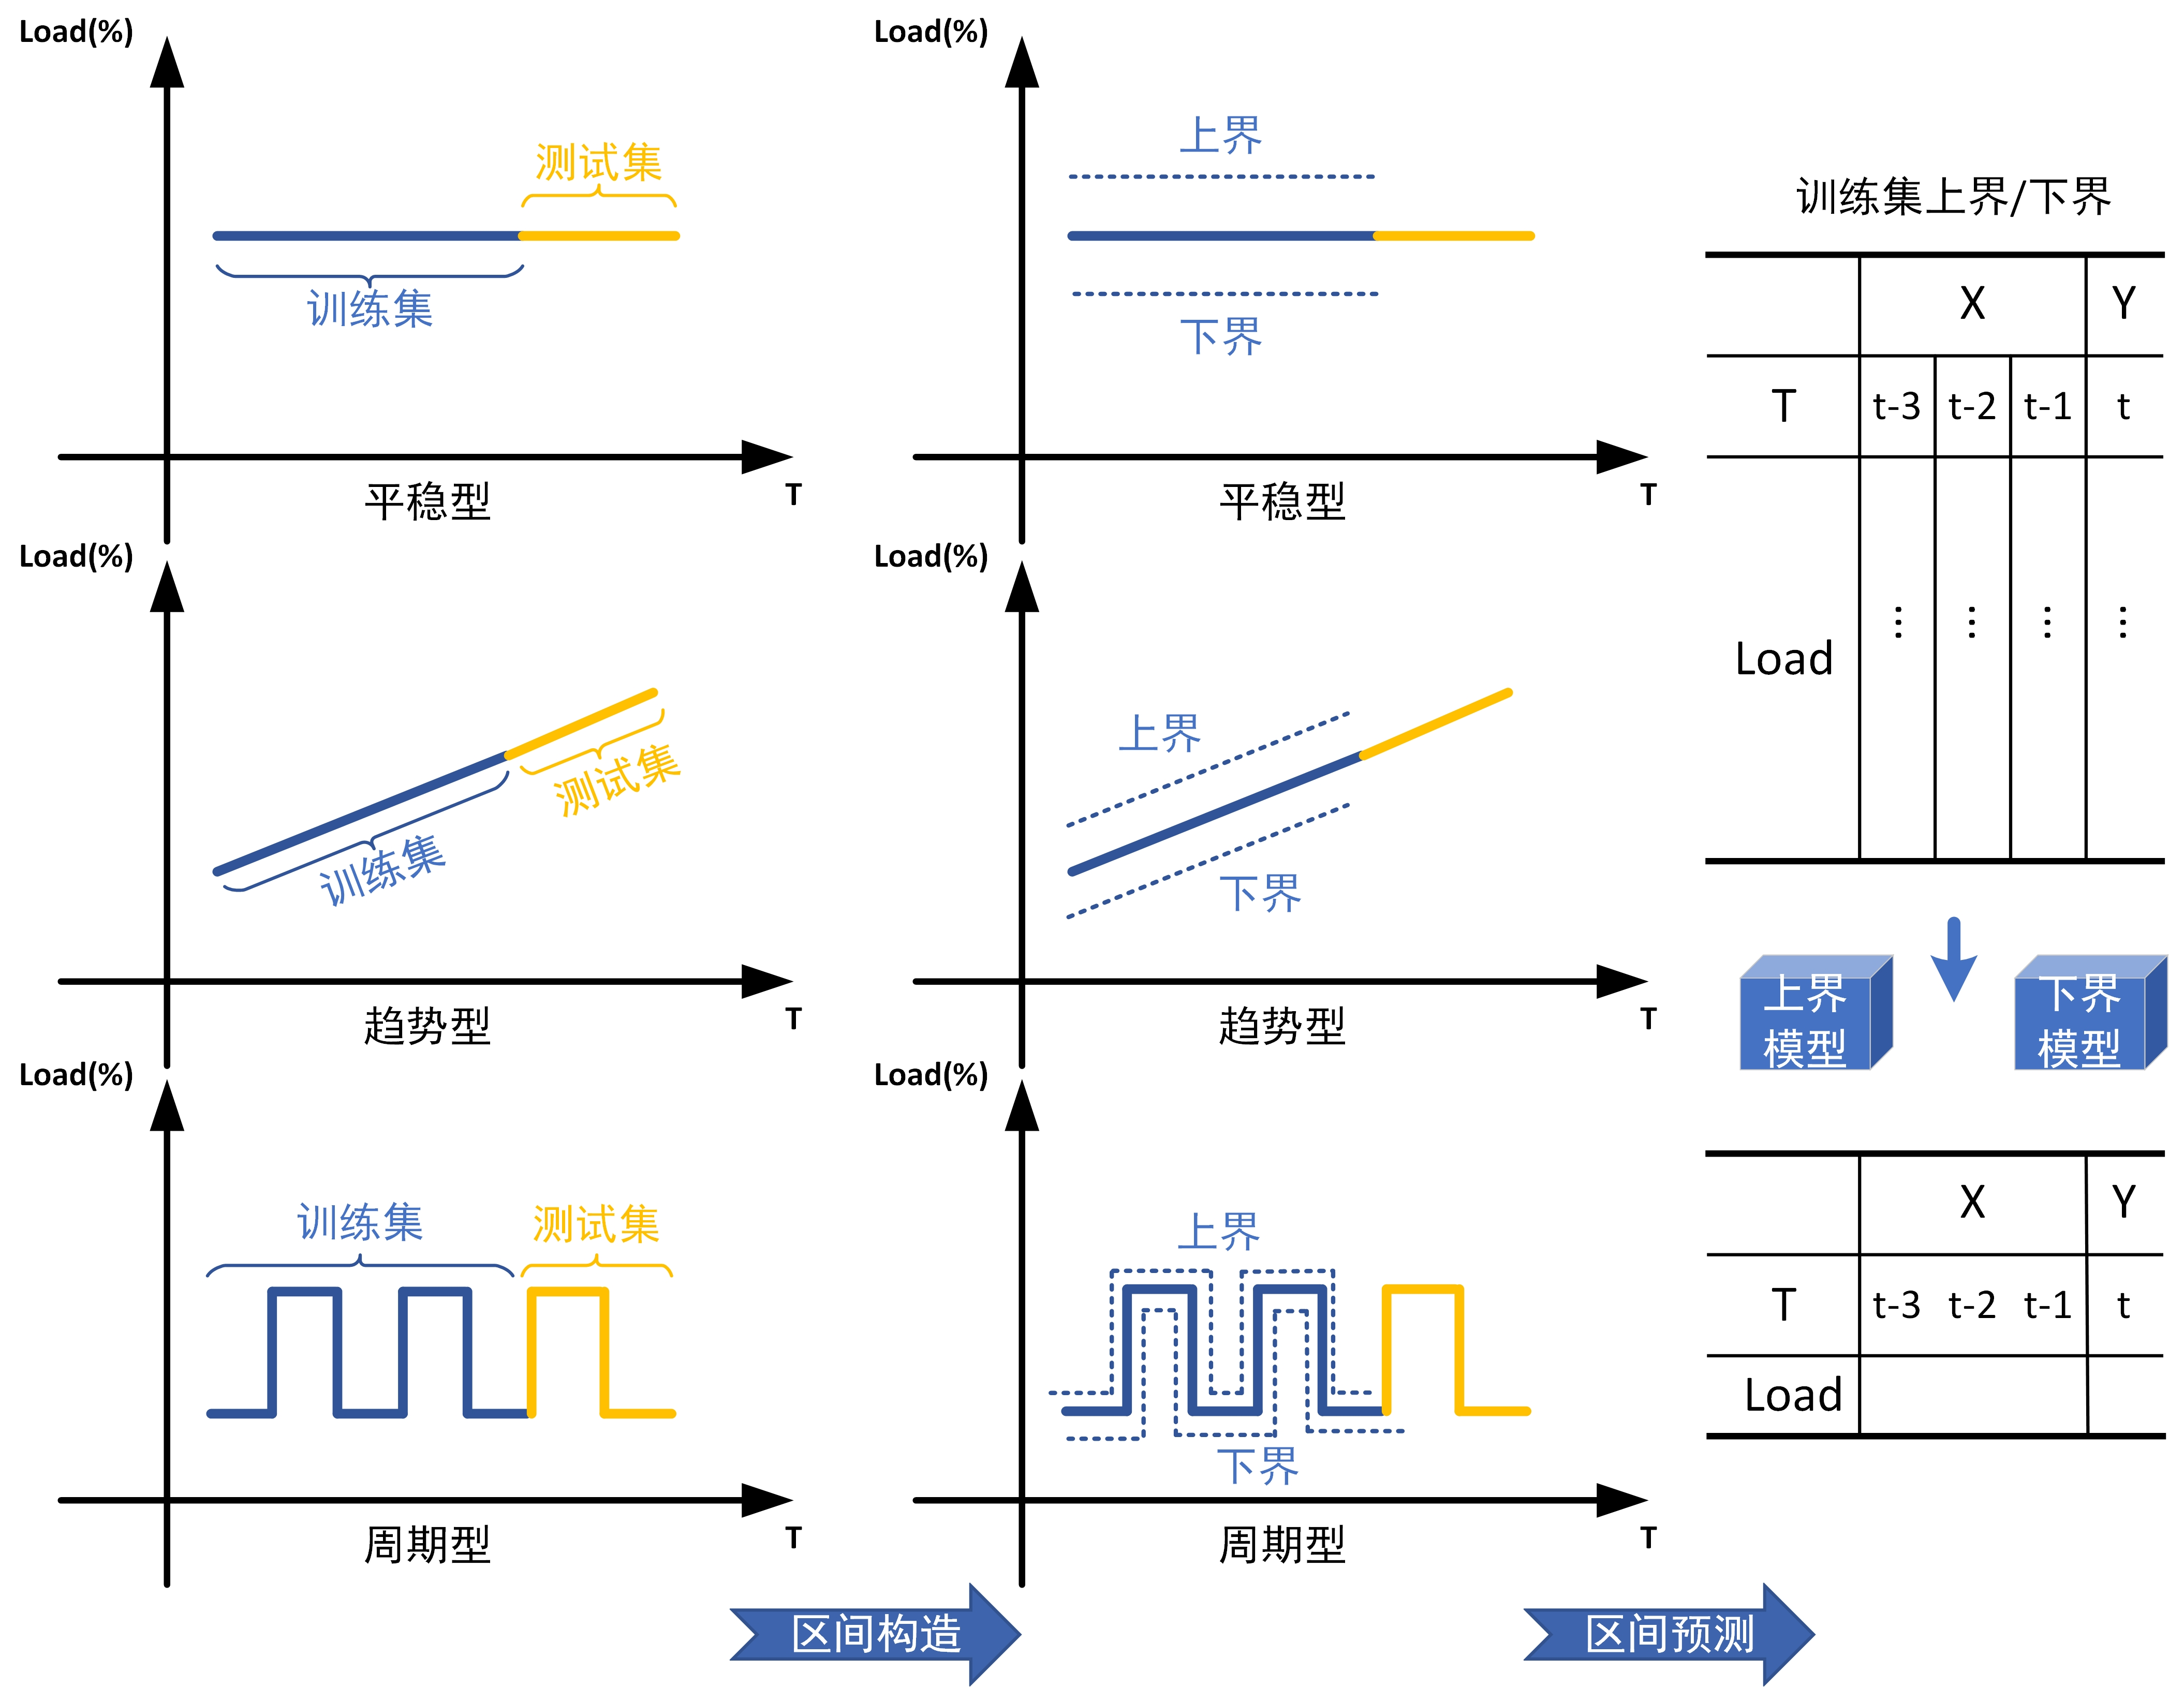
\includegraphics[scale=0.38]{figures/fig7_predict_process.jpg}
\caption{模型预测过程}
\label{fig:fig7}
\end{figure}
\end{column}
\end{columns}
\end{frame}

\subsection{趋势感知}

\begin{frame}
\frametitle{趋势感知}
\framesubtitle{定义}
\begin{itemize}
    \item 容器负载:\textbf{时间段$p$内CPU利用率均值}(\sout{Load Average})
    \begin{equation}
        load = avg(u(p))
    \end{equation}
    \item 负载时序数据
    \begin{equation}
        S=\{(t_1,load_1),(t_2,load_2),\cdots,(t_n,load_n)\}=\{(t_i,load_i)\}|^n_{i=1}
    \end{equation}
    \begin{equation}
        load_i = avg(u(t_i - t_{i-1}))
    \end{equation}
    \begin{itemize}
        \item $t_i - t_{i-1}$ \textbf{增大} $\Rightarrow$ \textbf{$load_i$ 平均特征}
        \item $t_i - t_{i-1}$ \textbf{减小} $\Rightarrow$ \textbf{$load_i$ 瞬时特征}
    \end{itemize}
\end{itemize}
\end{frame}

\begin{frame}
\frametitle{趋势感知}
\framesubtitle{SAC规则}
\begin{itemize}
    \item 频谱特征分析(\textbf{S}pectrum \textbf{A}nalysis)
    和自相关系数(\textbf{A}utocorrelation \textbf{C}oefficient)分析判定规则(SAC规则)
\end{itemize}
\begin{figure}[htb]
\centering
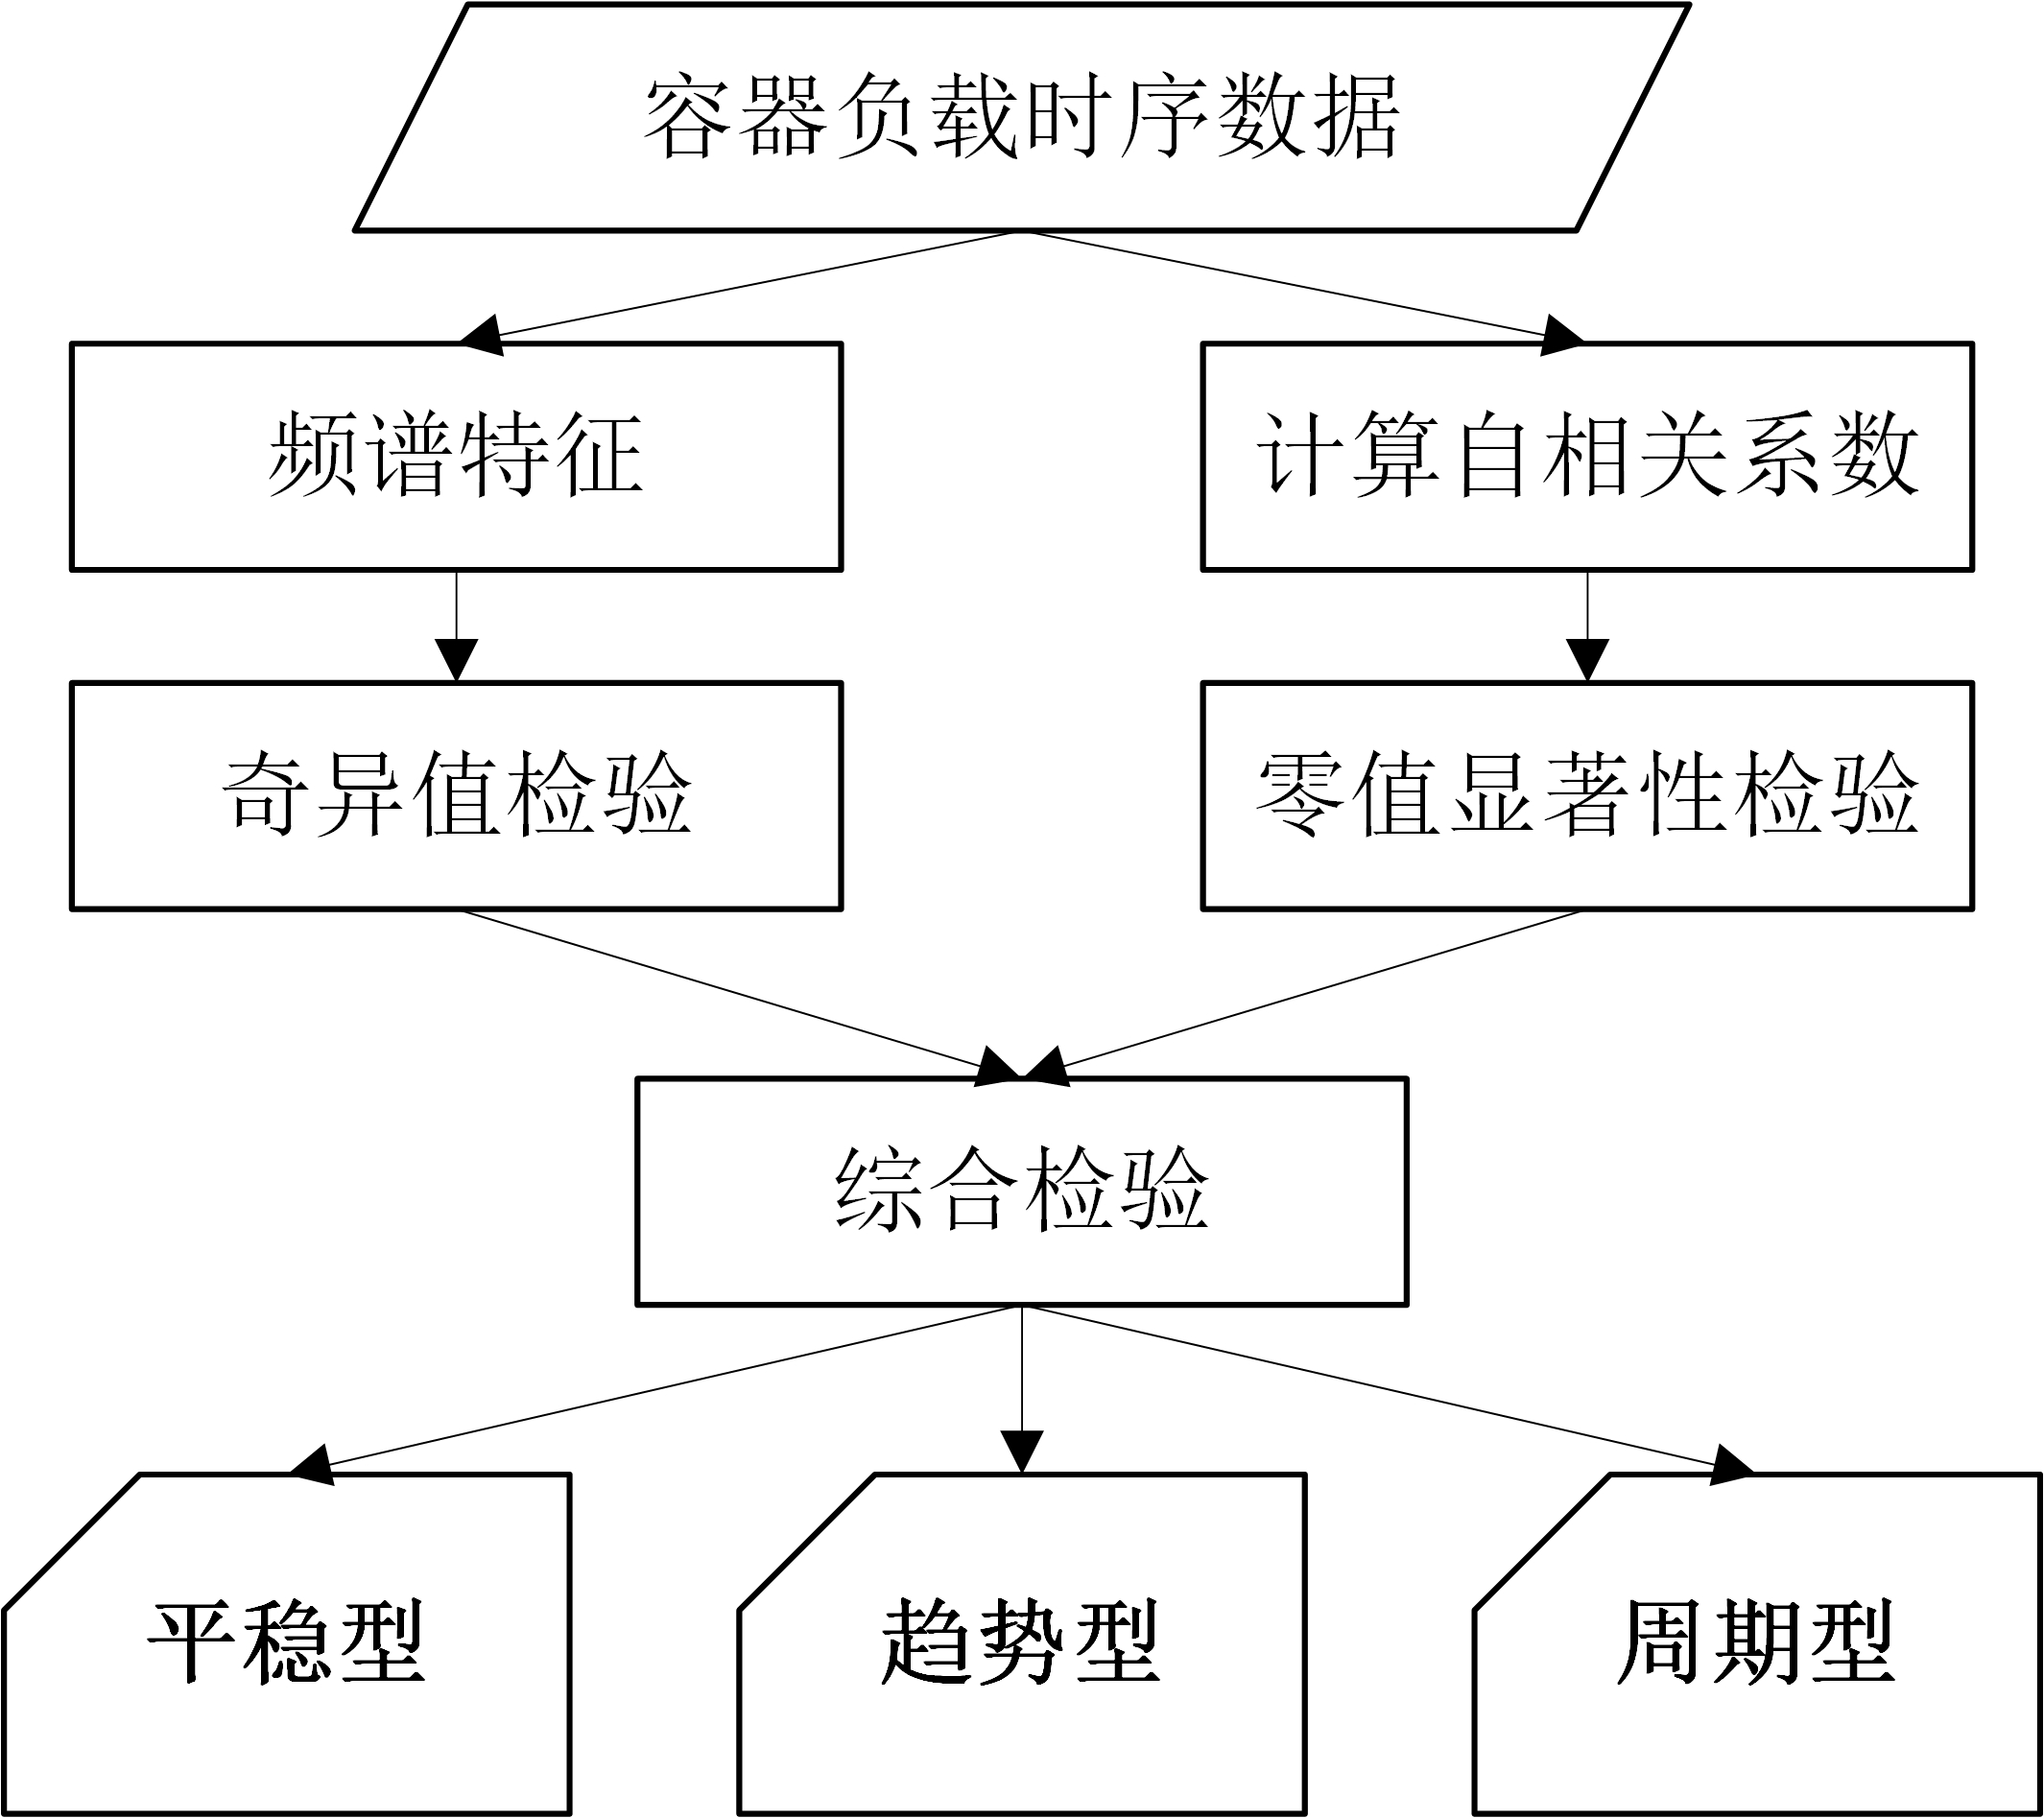
\includegraphics[scale=0.6]{figures/fig8_sac_process.jpg}
\caption{SAC规则实施流程}
\label{fig:fig8}
\end{figure}
\end{frame}

\begin{frame}
\frametitle{趋势感知}
\framesubtitle{SAC - 频谱特征分析}
\begin{enumerate}[1]
    \item 负载数据(\textbf{时域数据}) $\Rightarrow$ 负载信号(\textbf{频域数据})
    \item 频谱特征:负载信号表现出的特征
\end{enumerate}
\begin{block}{负载信号:某一采样频率下,负载在频域上的取值}
    \begin{itemize}
    \item 离散傅立叶变换(DFT)
    \end{itemize}
    \begin{equation}
    \left\{
        \begin{array}{rcl}
        F_{\color{red}{v}} &=& \sum_{j=1}^{n} e^{-i\frac{2\pi}{n}({\color{red}v}-1)(j-1)}load_i,
        {\color{red}v=1,2,\cdots,m} \\
        m &=& \lceil \frac{n}{2} \rceil
        \end{array}
    \right.
    \end{equation}
\end{block}
\begin{block}{频谱特征:如图\ref{fig:fig9}所示}
\begin{itemize}
    \item 单个频谱特征
    \begin{equation}
        q_v = \frac{1}{m}\left|F_v \right|^2,v=1,2,\cdots,m
    \end{equation}
    \item 频谱特征序列
    \begin{equation}
        Q = \{q_1,\cdots,q_m\} = \{q_v\}|^m_{v=1}
    \end{equation}
\end{itemize}
\end{block}
\bigskip
\end{frame}

\begin{frame}
\frametitle{趋势感知}
\framesubtitle{SAC - 频谱特征分析}
\begin{figure}[htb]
\centering
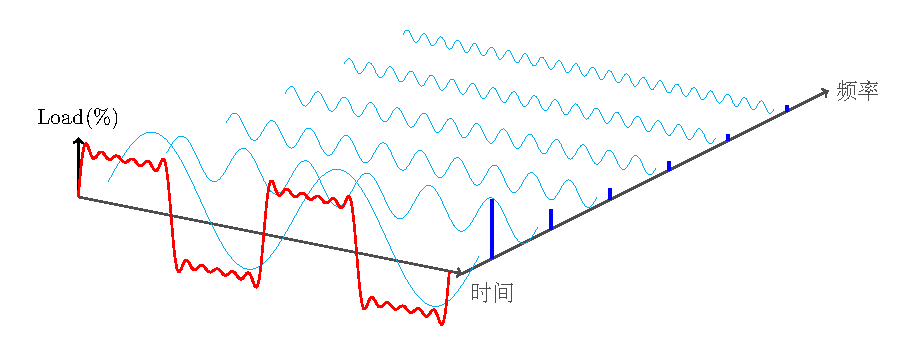
\includegraphics[scale=0.7]{figures/fig9_dft.pdf}
\caption{基于傅立叶变换的频谱特征分析原理示意图}
\label{fig:fig9}
\end{figure}
\end{frame}

\begin{frame}
\frametitle{趋势感知}
\framesubtitle{SAC - 自相关系数分析}
\begin{enumerate}[1]
    \item 按滞后期$k$,将原时序序列S拆分为两个新序列:$S_{before}$ 和 $S_{after}$
    \begin{itemize}
        \item 前置序列:$s_{before} = \{load_1,load_2,\cdots,load_{n-k}\}=\{load_i\}|^{n-k}_{i=1}$
        \item 后置序列:$s_{after} = \{load_{1+k},load_{2+k},\cdots,load_{n}\}=\{load_i\}|^{n}_{i=1+k}$
    \end{itemize}
    \item 计算滞后期为$k$时的自相关系数:$\bar{S} = \sum_{i=1}^{n} \frac{load_i}{n}$
    \begin{equation}
    \begin{aligned}
        \rho_k & =  \frac{\gamma(i,i+k)}{Var(S)} \\
               & = \frac{\sum_{i=1}^{n-k} (load_i - \bar{S})(load_{i+k} - \bar{S})}{\sum_{i=1}^{n} (load_i - \bar{S})^2}
    \end{aligned}
    \end{equation}
    \item 获得自相关系数序列:$k=1,2,\cdots,m$, $m = \lceil \frac{n}{3} \rceil$
    \begin{equation}
        P = \{\rho_1,\rho_2,\cdots,\rho_m\} = \{\rho_k\}|^m_{k=1}
    \end{equation}
\end{enumerate}
\bigskip
\end{frame}

\begin{frame}
\frametitle{趋势感知}
\framesubtitle{SAC - 判定}
    \begin{itemize}
        \item 周期性判定:奇异值检验
        \begin{enumerate}[1]
            \item 计算频谱特征序列$Q=\{q_v\}|^m_{v=1}$的差分序列$H = \{h_v\}|^{\lceil \frac{m}{2} \rceil}_{v=2}$
            \begin{equation}
                h_v = \left|(q_v - q_{v+1}) + (q_v - q_{v-1})\right|,v=2,3,\cdots,\lceil \frac{m}{2} \rceil
            \end{equation}
            \item 计算序列$H$的均值$\mu_H$和标准差$\sigma_H$
            \item $3\sigma$标准:序列$Q$中存在$q_v$使对应的差分项$h_v$满足如下条件
            \begin{equation}
                h_v - \mu_H > 3\sigma_H
                \label{eq:3sigma}
            \end{equation}
        \end{enumerate}
        \item 平稳性判定:显著性检验
        \begin{enumerate}[1]
            \item $t$-检验 $\Rightarrow$ H0:序列平稳,H1:序列不平稳,显著性水平:$\alpha=0.05$
            \item 计算自相关系数序列$P$总体与零值相关概率$P_\rho$
            \item 检验标准
            \begin{itemize}
                \item $P_\rho \geq \alpha$ $\Rightarrow$ 接受H0假设
                \item $P_\rho < \alpha$ $\Rightarrow$ 接受H1假设
            \end{itemize}
        \end{enumerate}
    \end{itemize}
\end{frame}

\begin{frame}
\frametitle{趋势感知}
\framesubtitle{SAC - 判定}
\begin{block}{负载类型定义}
    \begin{itemize}
        \item 平稳型负载:不存在$q_v$,使$h_v$满足公式\ref{eq:3sigma},且$P_\rho \geq \alpha$
        \item 趋势型负载:不存在$q_v$,使$h_v$满足公式\ref{eq:3sigma},且$P_\rho < \alpha$
        \item 周期型负载:存在$q_v$,使$h_v$满足公式\ref{eq:3sigma}
    \end{itemize}
\end{block}
\end{frame}

\subsection{区间构造}

\begin{frame}
\frametitle{区间构造}
\framesubtitle{平稳型}
\begin{itemize}
    \item \textbf{区间构造算法 - 平稳型负载}
\end{itemize}
%\begin{block}{平稳型负载}
\begin{algorithmic}[1]
  \Require{$S$, $Type$, $Period$}
  \Ensure{$S_u$, $S_l$}
    \State $S_{max} =$ max($S$), $S_{min} =$ min($S$), $S_{len} =$ length($S$)
    \If{$Type ==$ \textbf{TYPE\_SMOOTH}}
      \For{$i=1$, $i \leq S_{len}$; $i$++}
        \State $S_u$.add($0.5*(S_i + S_{max})$) \Comment{构建上界}
        \State $S_l$.add($0.5*(S_i + S_{min})$) \Comment{构建下界}
      \EndFor
    \EndIf \\
    \Return $S_u$, $S_l$
\end{algorithmic}
%\end{block}
\end{frame}

\begin{frame}[allowframebreaks]
\frametitle{区间构造}
\framesubtitle{趋势型}
\begin{itemize}
    \item \textbf{区间构造算法 - 趋势型负载}
\end{itemize}
\begin{algorithmic}[1]
\Require{$S$, $Type$, $Period$}
\Ensure{$S_u$, $S_l$}
  \State $S_{max} =$ max($S$), $S_{min} =$ min($S$), $S_{len} =$ length($S$)
  \If{$Type ==$ \textbf{TYPE\_TENDENCY}}
    \For{$i=1$; $i \leq S_{len}$; $i$++} \Comment{差分项均值 $\Rightarrow$ 活动空间}
      \State $interval$.add(abs($S_{i+1} - S_i$))
    \State $interval\_avg =$ average($interval$)
    \EndFor
    \framebreak
    \For{$i=1$; $i \leq S_{len}$; $i$++} \Comment{增长趋势 $\Rightarrow$ 构建区间}
      \If{$tendency ==$ \textbf{UP}}
        \State $S_u$.add($S_i + interval\_avg + (S_{max} - S_i)/(S_{len} - i)$)
        \State $S_l$.add($S_i - interval\_avg$)
      \EndIf
      \If{$tendency ==$ \textbf{LOW}} \Comment{下降趋势 $\Rightarrow$ 构建区间}
        \State $S_u$.add($S_i + interval\_avg $)
        \State $S_l$.add($S_i - interval\_avg - (S_i - S_{min})/(S_{len} - i)$)
      \EndIf
    \EndFor
  \EndIf \\
  \Return $S_u$, $S_l$
\end{algorithmic}
\bigskip
\end{frame}

\begin{frame}[allowframebreaks]
\frametitle{区间构造}
\framesubtitle{周期型}
\begin{itemize}
    \item \textbf{区间构造算法 - 周期型负载}
\end{itemize}
\begin{algorithmic}[1]
  \Require{$S$, $Type$, $Period$}
  \Ensure{$S_u$, $S_l$}
    \State $S_{max} =$ max($S$), $S_{min} =$ min($S$), $S_{len} =$ length($S$)
    \If{$Type ==$ \textbf{TYPE\_PERIOD}}
      \For{$i=1$; $i \leq S_{len}$; $i$++} \\
        \Comment{周期前段️ $\Rightarrow$ 活动空间}
        \If{$i \leq $ int($Period/2$) $+1$}
          \For{$j=1$; $j \leq (Period - 1)$; $j$++}
            \State $interval$.add(abs($S_{j+1}-S_j$))
            \State $interval\_avg =$ average($interval$)
          \EndFor
        \EndIf
        \framebreak \\
        \Comment{周期中段️ $\Rightarrow$ 活动空间}
        \If{int($Period/2$) $+ 1 < i < S_{len} - ($int($Period/2$)$-1)$}
          \For{$j=i-$ int($Period/2$); $j \leq i+$ int($Period/2$) $-1$; $j$++}
            \State $interval$.add(abs($S_{j+1}-S{j}$))
            \State $interval\_avg =$ average($interval$)
          \EndFor
        \EndIf \\
        \Comment{周期后段️ $\Rightarrow$ 活动空间}
        \If{$i \geq S_{len} - $ (int($Period/2$) $-1$)}
          \For{$i=S_{len} - Period$; $j \leq S_{len} - 1$; $j$++}
                    \State $interval$.add(abs($S_{j+1}-S{j}$))
                    \State $interval\_avg =$ average($interval$)
                  \EndFor
        \EndIf \\
        \framebreak
        \State $S_u$.add($S_i + interval\_avg$) \Comment{构建上界}
        \State $S_i$.add($S_i - interval\_avg$) \Comment{构建下界}
      \EndFor
    \EndIf \\
    \Return $S_u$, $S_l$
\end{algorithmic}
\end{frame}

\subsection{区间预测}

\begin{frame}[allowframebreaks]
\frametitle{区间预测}
\framesubtitle{超参数优化}
\begin{itemize}
    \item 用带梯度信息的粒子群算法来优化SVM模型:\textbf{GPSO-SVM}
\end{itemize}
\begin{algorithmic}[1]
  \Require{$S^u_{train}$, $S^l_{train}$}
  \Ensure{$C^u_{gbest}$, $\gamma^u_{gbest}$, $C^l_{gbest}$, $\gamma^l_{gbest}$}
  \State init($particles_{max}$, $iterator_{max}$, $position$, $velocity$)
  \State $trainBag_u$, $testBag_u$ = fold($S^u_{train}$, $5$)
  \State $trainBag_l$, $testBag_l$ = fold($S^l_{train}$, $5$)
  \For{$i=1$; $i \leq iterator_{max}$; $i$++}
    \\
    \Comment{计算粒子\textbf{适应度}与\textbf{梯度信息}}
	\State $C^u$, $\gamma^u$, $C^l$, $\gamma^l$ = PSO(SVM($trainBag_u$, $testBag_u$, $trainBag_l$, $testBag_l$))
	\\
	\Comment{适应度函数 - \alert{\textbf{CWC}}}
	\State $fitness$ = CWC($C^u$, $\gamma^u$, $C^l$, $\gamma^l$, $trainBag_u$, $testBag_u$, $trainBag_l$, $testBag_l$)
	\\
	\Comment{梯度信息 - \textbf{粒子向最优运动的方向\ \ \ \ \ \ \ }}
	\State $G$ = gradient()
	\framebreak
	\If{$fitness < fitness_{lbest}$} \Comment{更新\textbf{局部最优}}
		\State $fitness_{lbest}$ = $fitness$
		\State $C^u_{lbest}$, $\gamma^u_{lbest}$, $C^l_{lbest}$, $\gamma^l_{lbest}$ = $C^u$, $\gamma^u$, $C^l$, $\gamma^l$
	\EndIf
	\If{$fitness_{lbest} < fitness_{gbest}$} \Comment{更新\textbf{全局最优}}
		\State $fitness_{gbest}$ = $fitness_{lbest}$
		\State $C^u_{gbest}$, $\gamma^u_{gbest}$, $C^l_{gbest}$, $\gamma^l_{gbest}$ = $C^u_{lbest}$, $\gamma^u_{lbest}$, $C^l_{lbest}$, $\gamma^l_{lbest}$
	\EndIf
	\State $position$, $velocity$ = update($position$, $velocity$)
  \EndFor \\
  \Return $C^u_{gbest}$, $\gamma^u_{gbest}$, $C^l_{gbest}$, $\gamma^l_{gbest}$
\end{algorithmic}
\end{frame}

\begin{frame}
\frametitle{区间预测}
\framesubtitle{CWC标准}
\begin{itemize}
    \item<1-> 区间覆盖度标准(Coverage Width Criterion, CWC)
    \begin{itemize}
        \item<1> \scriptsize{预测区间覆盖率(Prediction Interval Coverage Probability, PICP)}
        \begin{equation}
        \begin{aligned}
            PICP &= \frac{1}{N} \sum_{i=1}^{N} C_i \\
            \text{where } C_i &=
                \left\{
                    \begin{array}{rcl}
                    1 \ t_i \in [L_i,U_i] \\
                    0 \ t_i \notin [L_i,U_i]
                    \end{array}
                \right.
        \end{aligned}
        \end{equation}
        \item<1> \scriptsize{预测区间归一化平均宽度(Prediction Interval Normalized Average Width, PINAW)}
        \begin{equation}
            PINEW = \frac{1}{rN} \sum_{i=1}^{N} (U_i - L_i)
        \end{equation}
    \end{itemize}
    \visible<2>{
    \begin{equation}
        \begin{aligned}
            CWC &= PINAW * (1 + \gamma e^{\eta(PICP-\mu)}) \\
            \text{where } \gamma &=
                            \left\{
                                \begin{array}{rcl}
                                0 \ PICP \geq \mu \\
                                1 \ PICP < \mu
                                \end{array}
                            \right.
        \end{aligned}
    \end{equation}}
\end{itemize}
\bigskip
\end{frame}


\begin{frame}
\frametitle{区间预测}
\framesubtitle{训练与预测}
\begin{itemize}
    \item 基于最优参数SVM模型:$C^u_{gbest}$, $\gamma^u_{gbest}$, $C^l_{gbest}$, $\gamma^l_{gbest}$
\end{itemize}
\begin{algorithmic}[1]
\Require{$C^u_{gbest}$, $\gamma^u_{gbest}$, $C^l_{gbest}$, $\gamma^l_{gbest}$, $S^u_{train}$, $S^l_{train}$, $S^u_{test}$, $S^l_{test}$}
\Ensure{$P^u$, $P^l$}
    \\
    \Comment{基于最优超参数的\textbf{上界模型}}
    \State $svm_u$ = SVM($kernel$=\textbf{RBF}, $C$=$C^u_{gbest}$, $\gamma$=$\gamma^u_{gbest}$)
    \State $model_u =$ $svm_u$.fit($S^u_{train}$) \Comment{训练模型}
    \State $P^u =$ $model_u$.predict($S^u_{test}$.Time) \Comment{预测上界}
    \\
    \Comment{基于最优超参数的\textbf{下界模型}}
    \State $svm_l$ = SVM($kernel$=\textbf{RBF}, $C$=$C^l_{gbest}$, $\gamma$=$\gamma^l_{gbest}$)
    \State $model_l =$ $svm_l$.fit($S^l_{train}$) \Comment{训练模型}
    \State $P^l =$ $model_l$.predict($S^l_{test}$.Time) \Comment{预测下界}\\
    \Return{$P^u$, $P^l$}
\end{algorithmic}
\end{frame}

\subsection{实验结果与分析}

\begin{frame}
\frametitle{实验结果与分析}
\framesubtitle{预测效果分析}
\begin{itemize}
    \item SAC-GPSO-SVM模型预测效果:数据来源(PlanetLab)\footnote{\tiny{2011.03.03-2011.04.20内11746个容器当日每5分钟内CPU利用率均值数据}}
\end{itemize}
\begin{minipage}{\textwidth}
    \centering
    \begin{figure}[htb]
    \centering
    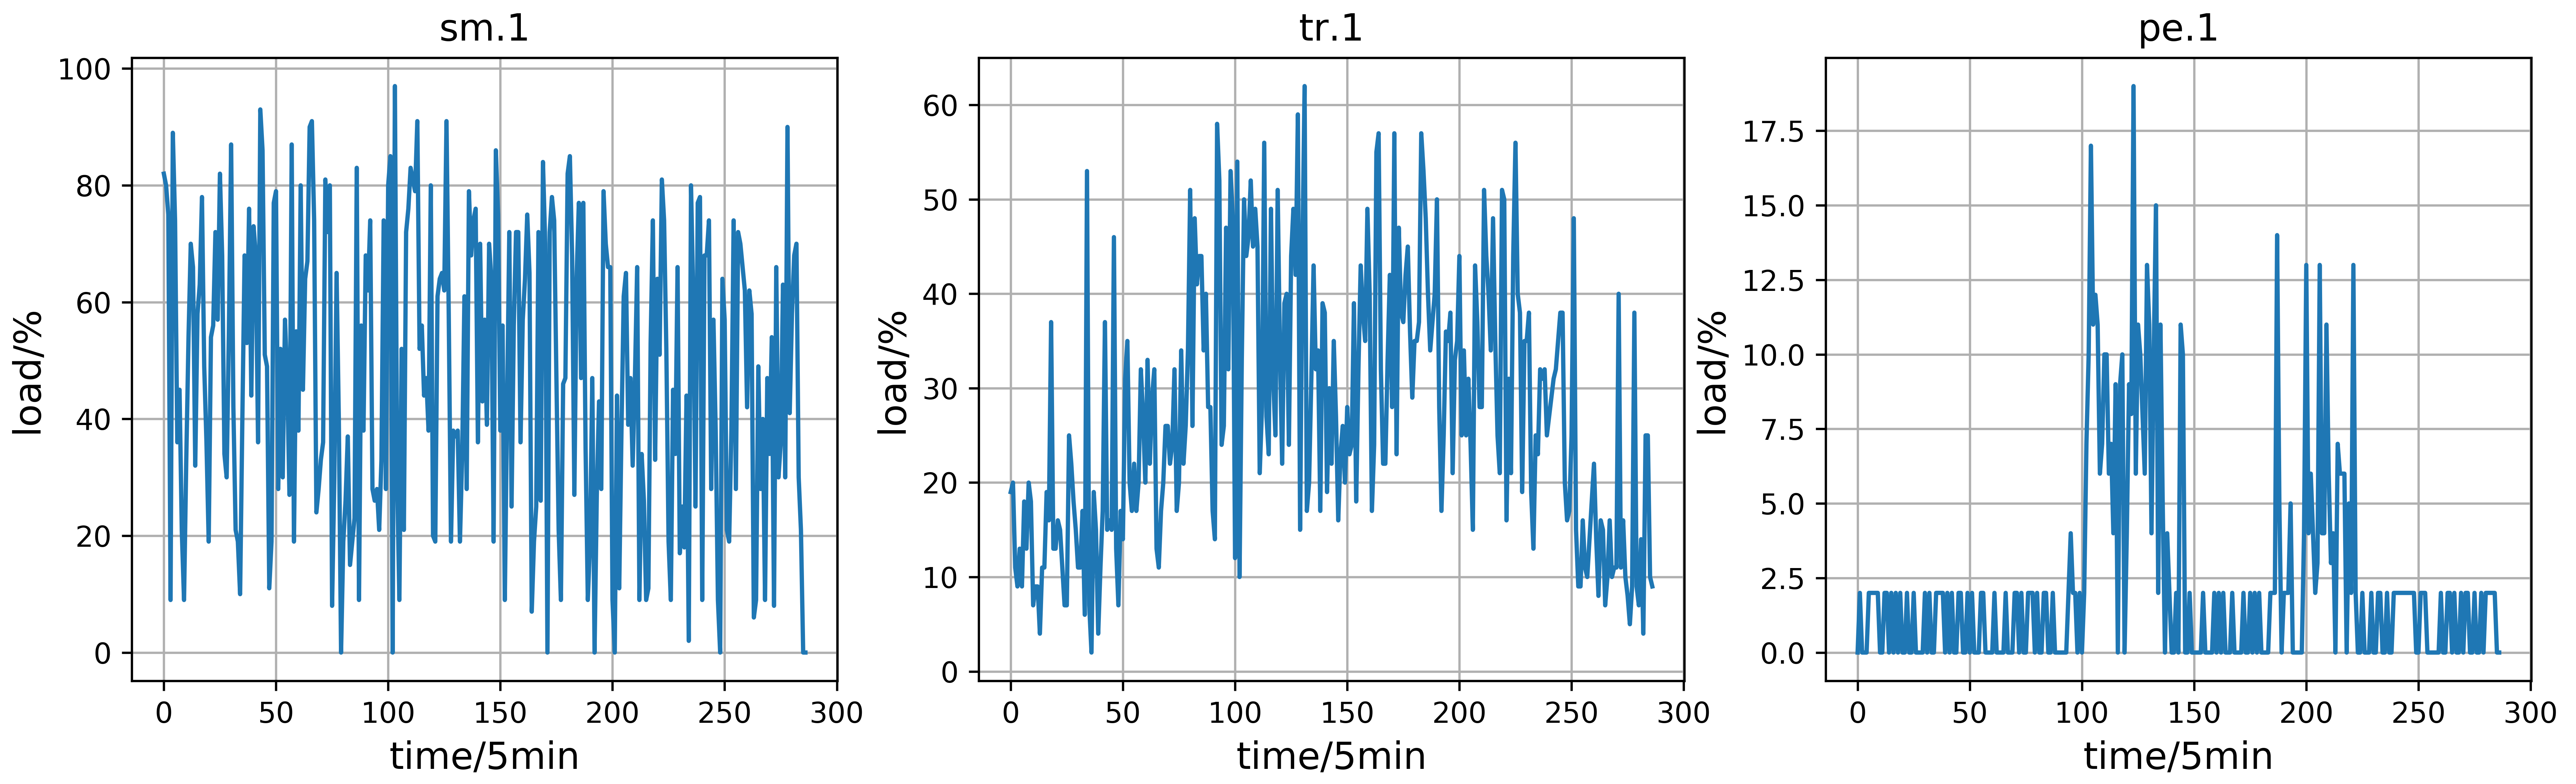
\includegraphics[width=0.8\textwidth]{figures/fig10_data_of_sm_tr_pe.png}
    \caption{平稳型、趋势型和周期型容器24h/5min的负载数据}
    \label{fig:fig10}
    \end{figure}
\end{minipage}
\begin{columns}[T,onlytextwidth]
\begin{column}{0.3\textwidth}
    \begin{minipage}{\textwidth}
        \begin{figure}
        \centering
        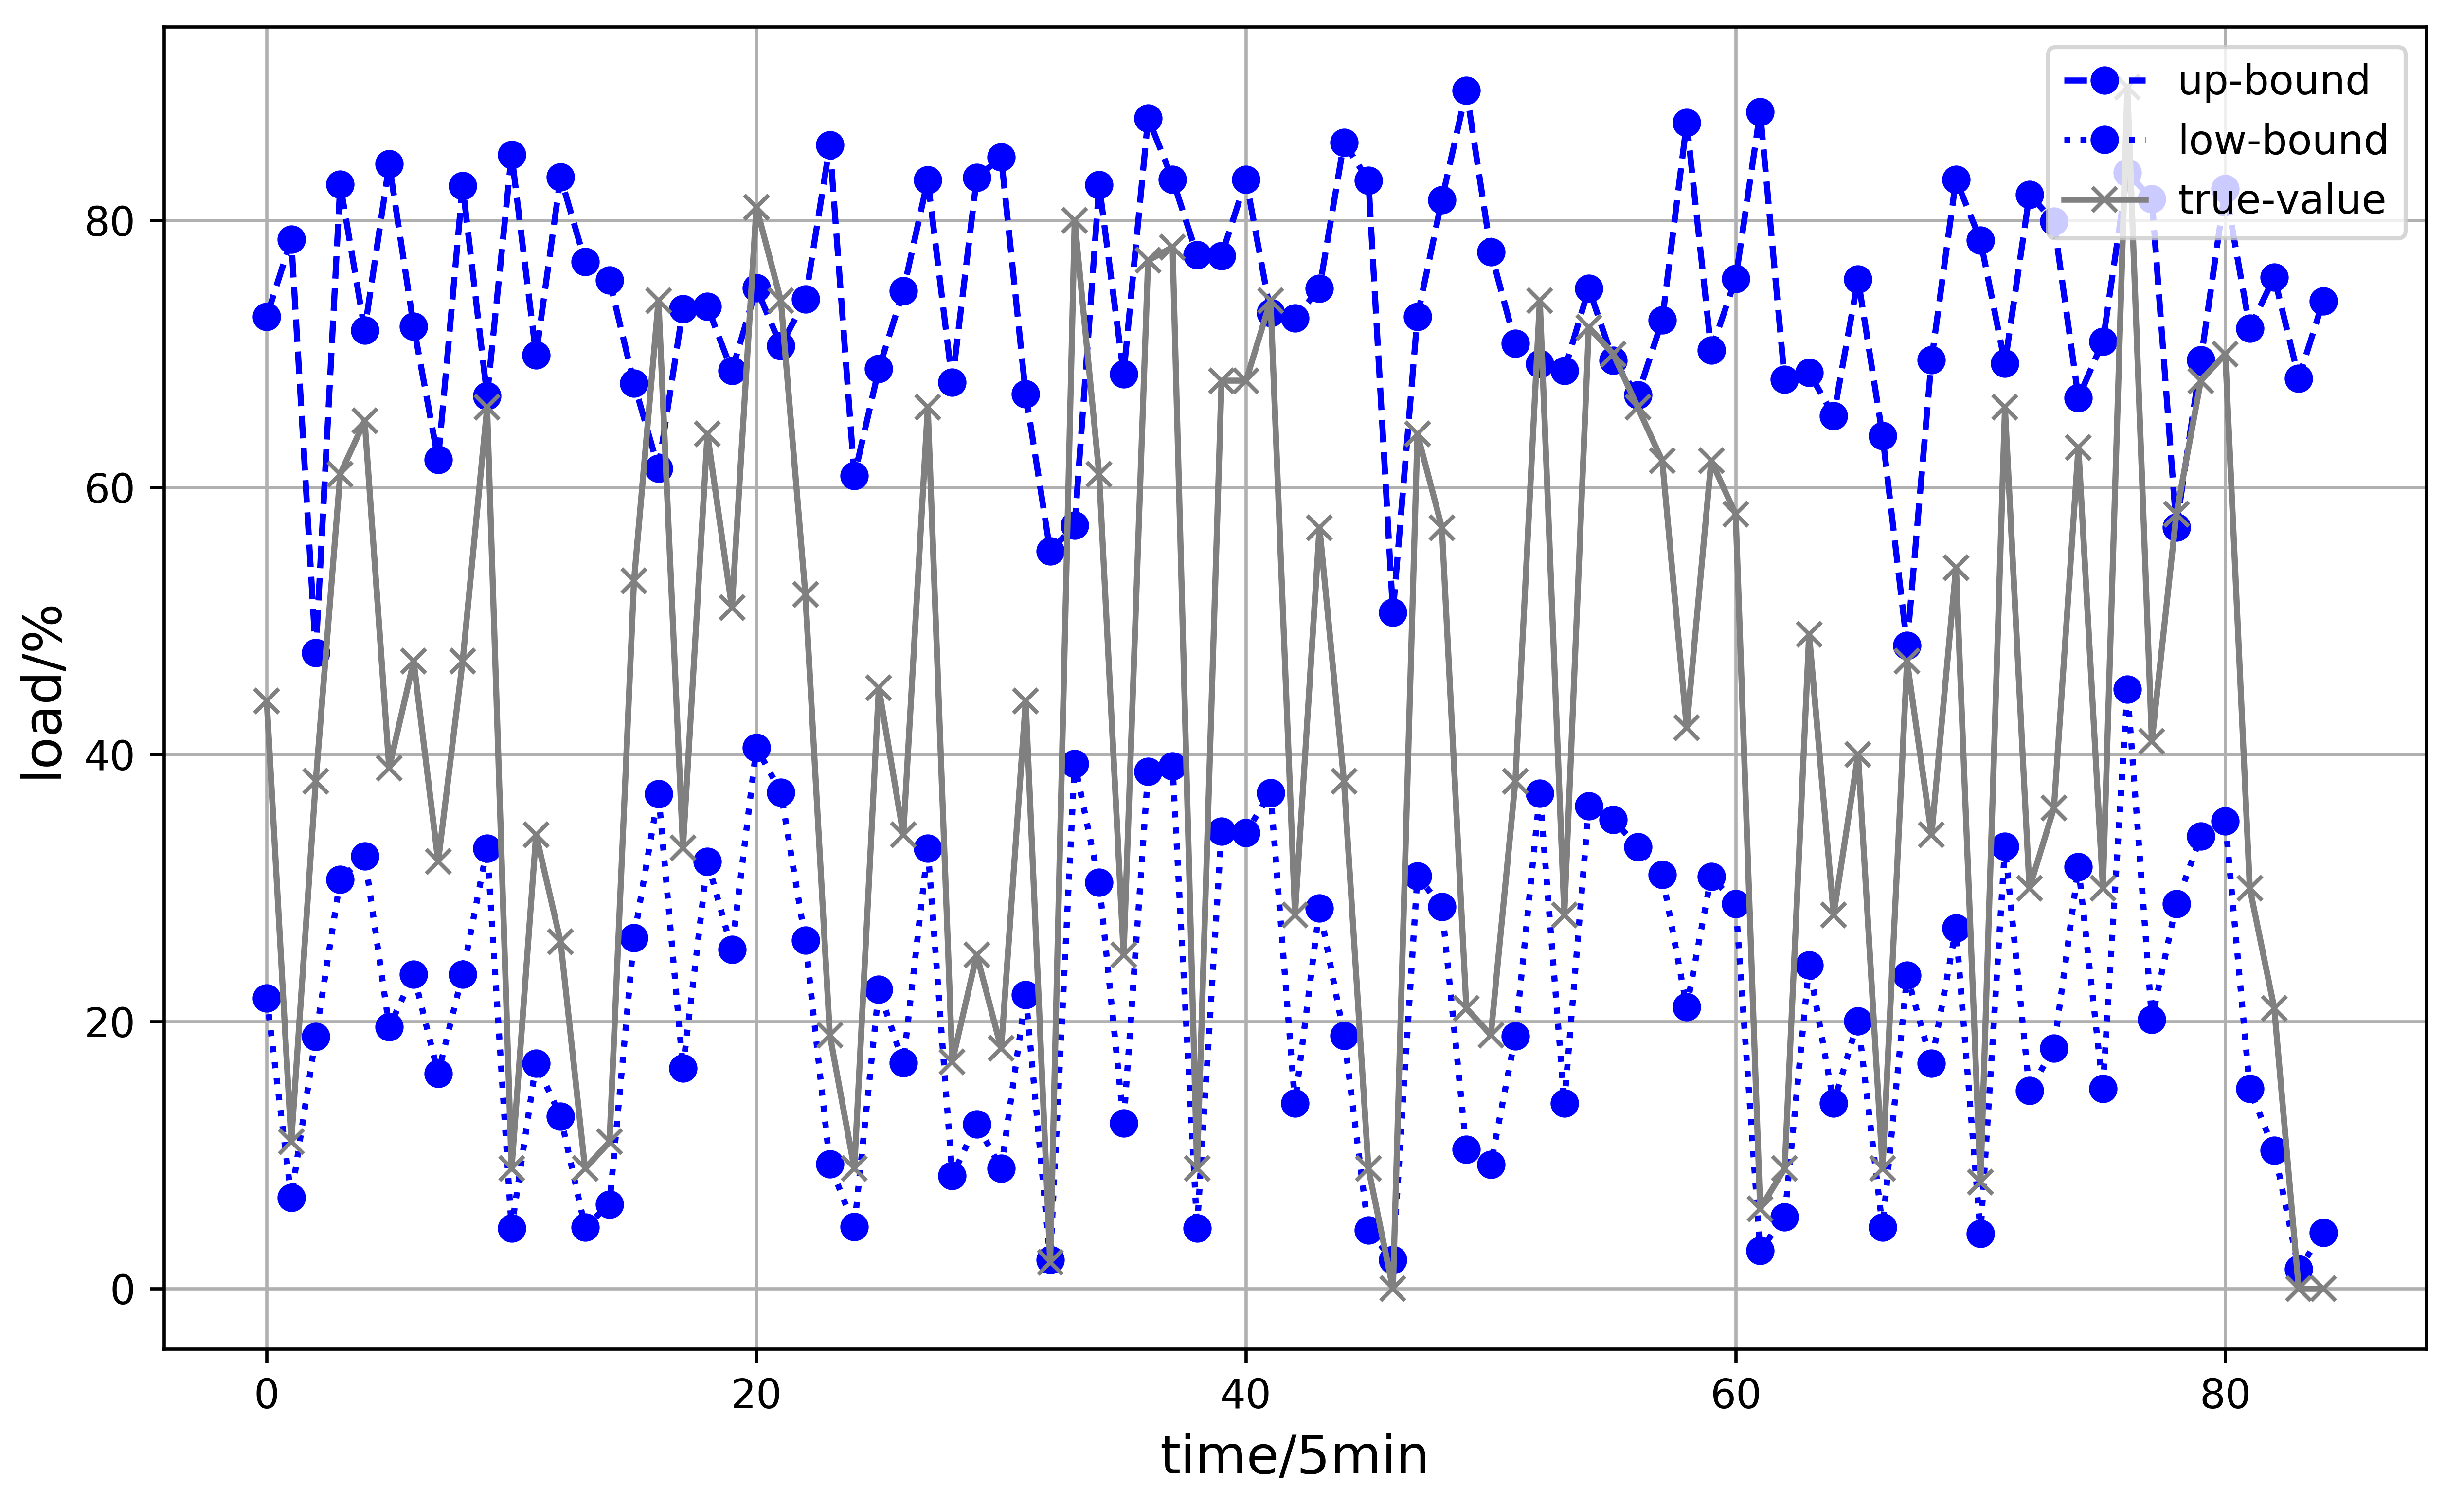
\includegraphics[width=\textwidth]{figures/fig11_a_sm_predict.png}
        \caption{sm.1预测结果}
        \label{fig:fig11_a}
        \end{figure}
    \end{minipage}
\end{column}
\begin{column}{0.3\textwidth}
    \begin{minipage}{\textwidth}
        \begin{figure}
        \centering
        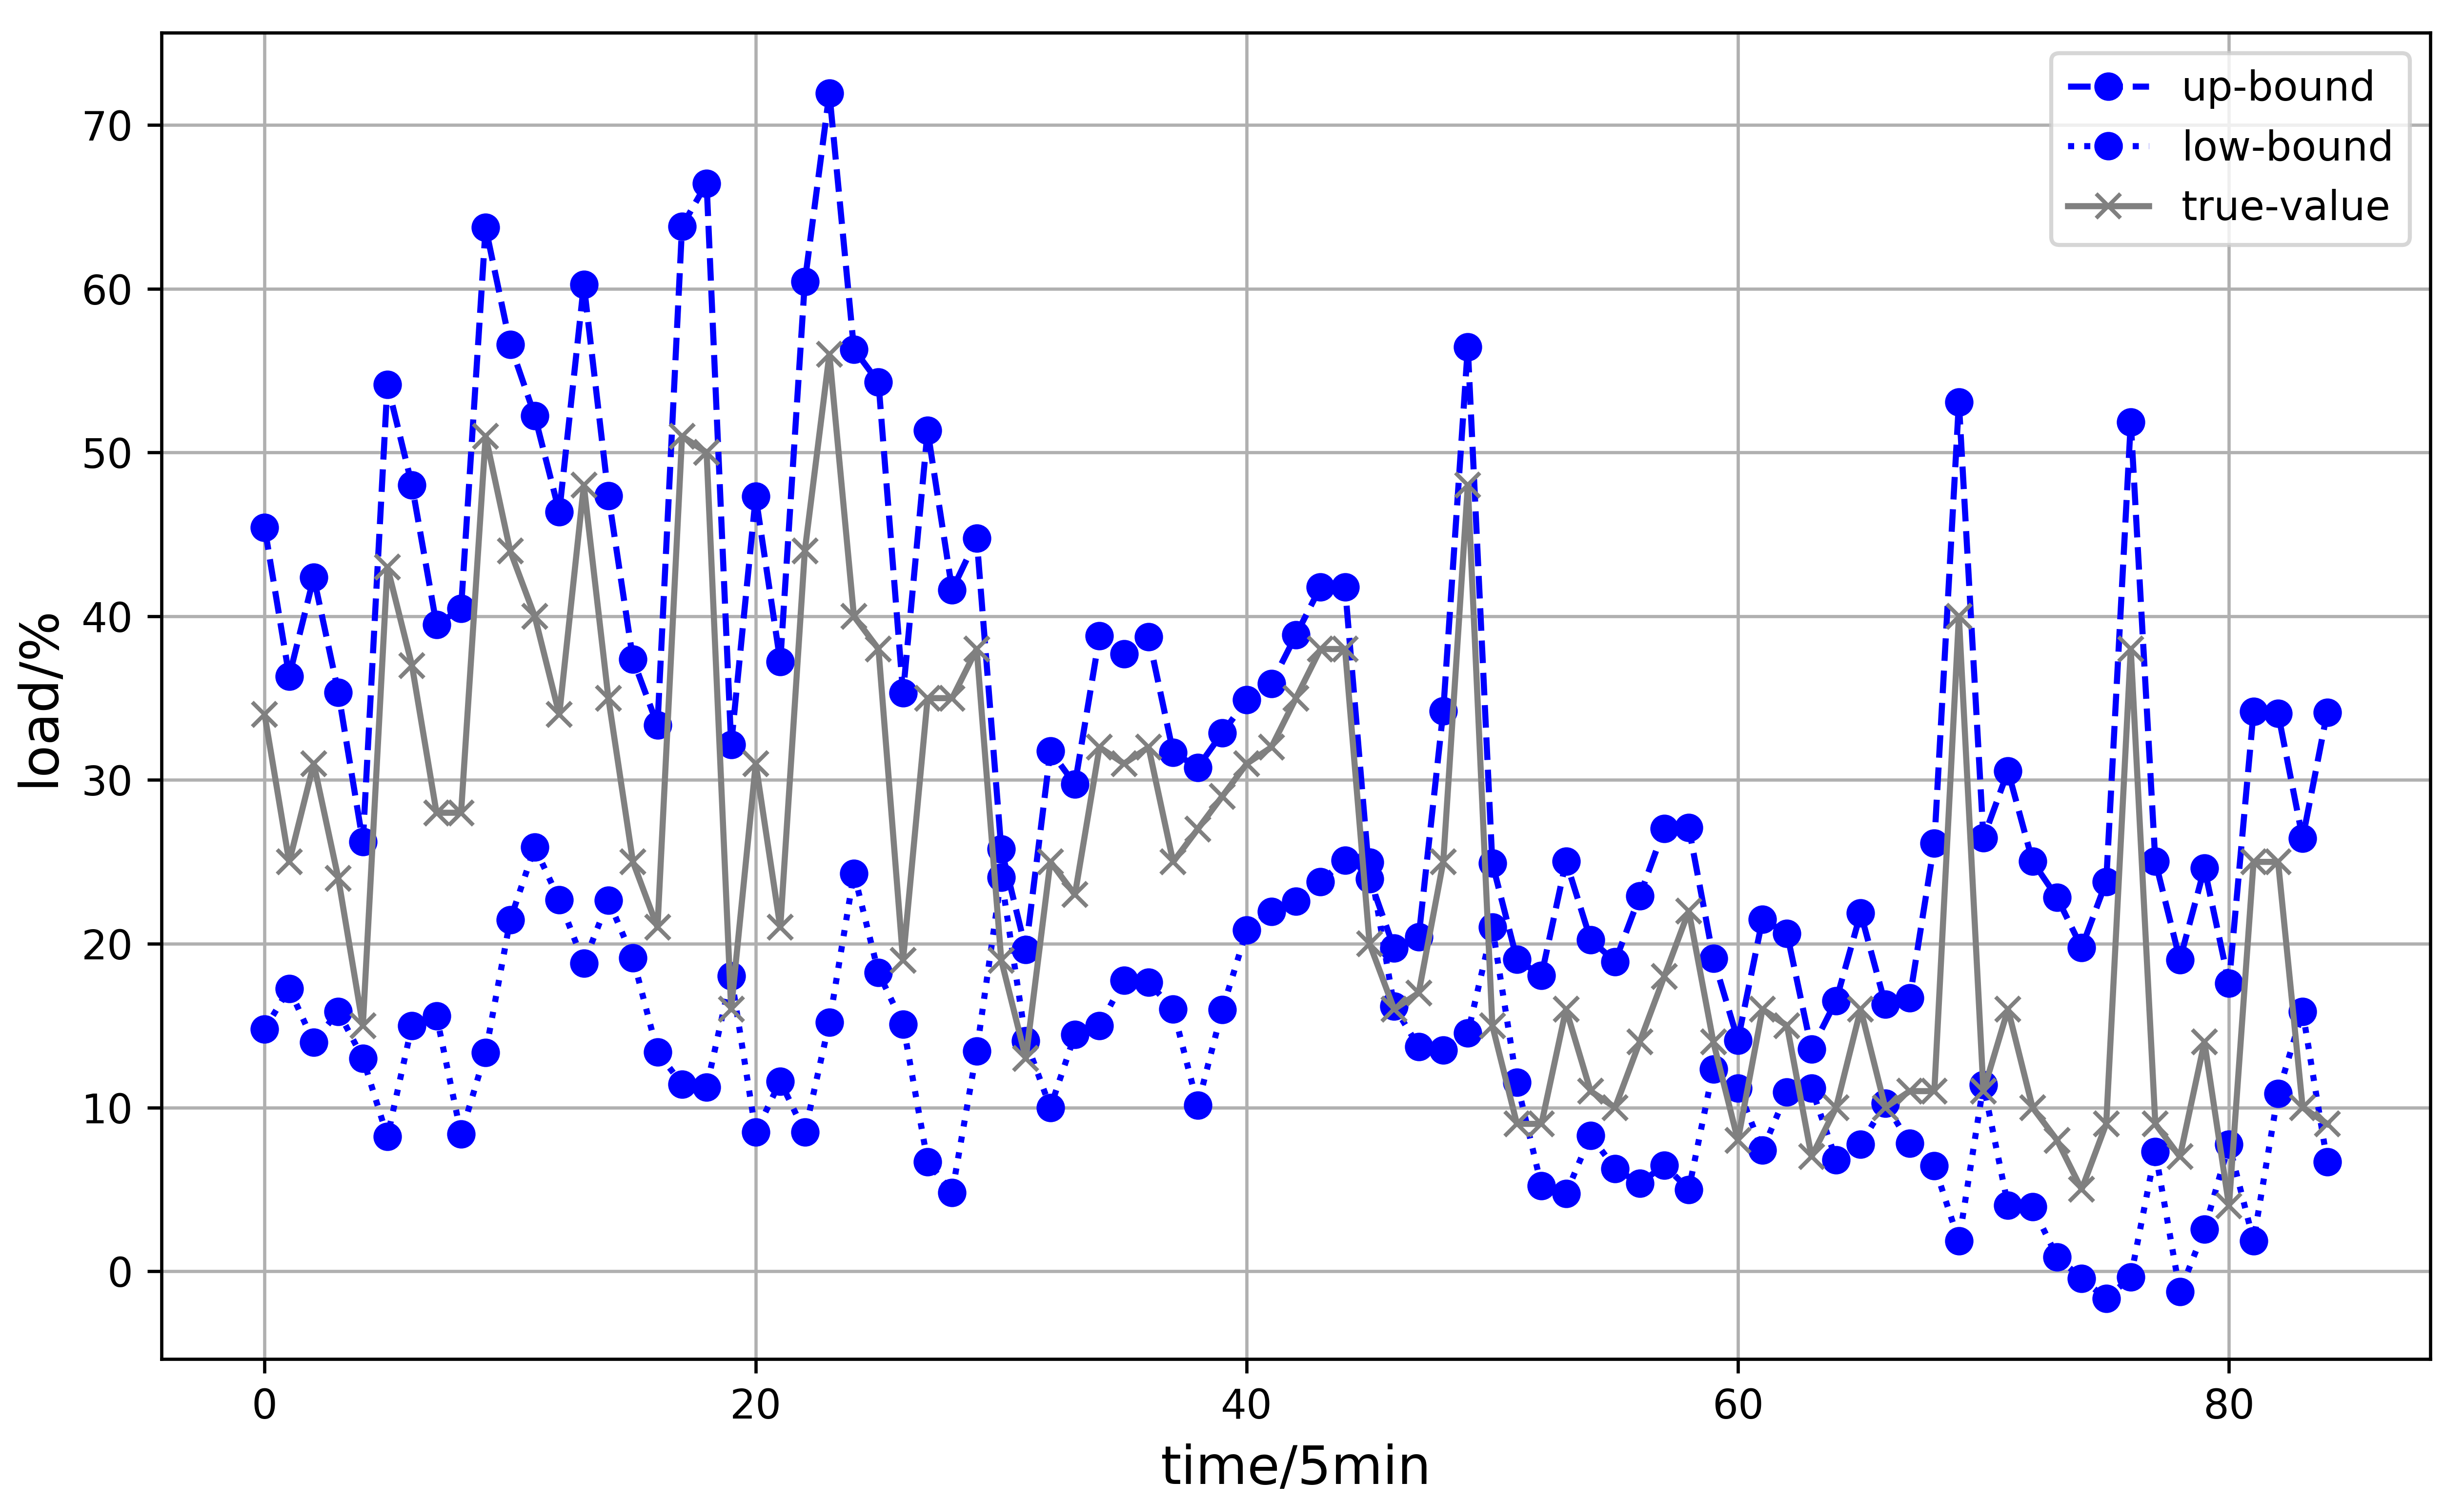
\includegraphics[width=\textwidth]{figures/fig11_b_tr_predict.png}
        \caption{tr.1预测结果}
        \label{fig:fig11_b}
        \end{figure}
    \end{minipage}
\end{column}
\begin{column}{0.3\textwidth}
    \begin{minipage}{\textwidth}
        \begin{figure}
        \centering
        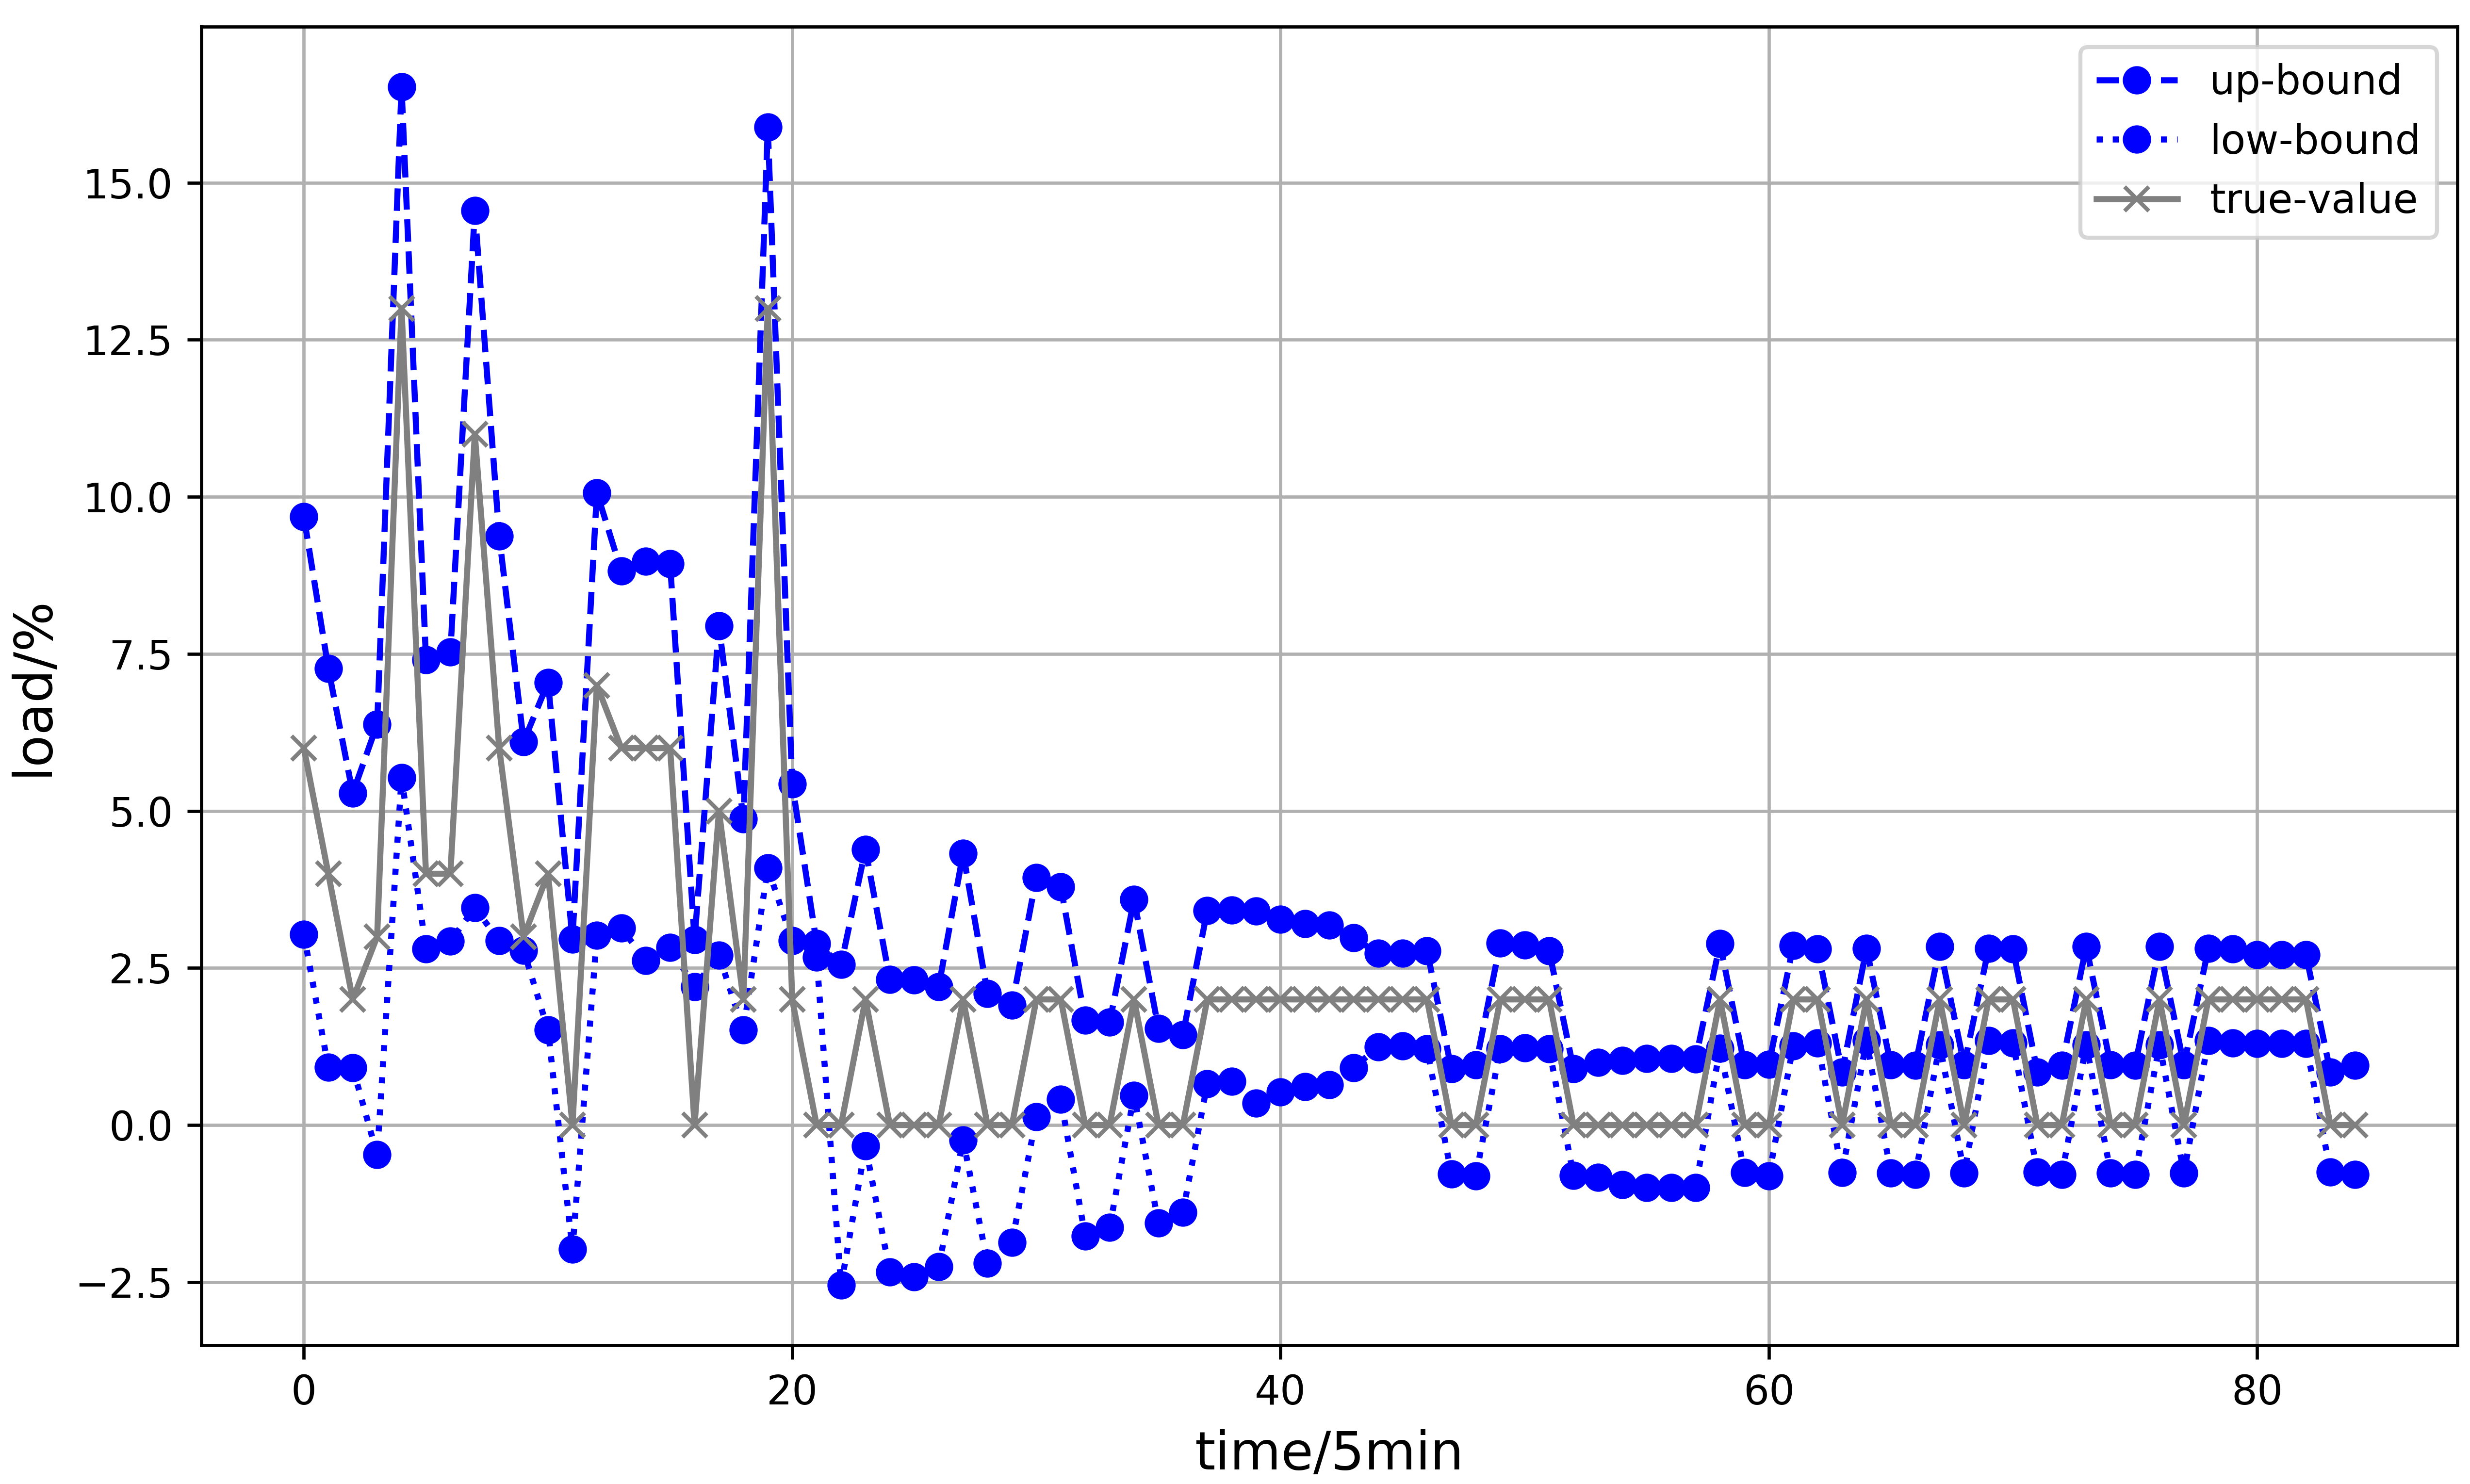
\includegraphics[width=\textwidth]{figures/fig11_c_pe_predict.png}
        \caption{pe.1预测结果}
        \label{fig:fig11_c}
        \end{figure}
    \end{minipage}
\end{column}
\end{columns}
\end{frame}


\begin{frame}
\frametitle{实验结果与分析}
\framesubtitle{预测效果分析}
\begin{block}{对比算法}
    \begin{itemize}
        \item Native Bayes,Linear Regression,SVM,CART和RFR
    \end{itemize}
\end{block}
\begin{itemize}
    \item Native Bayes
\end{itemize}
\begin{minipage}{\textwidth}
    \centering
    \begin{figure}[htb]
    \centering
    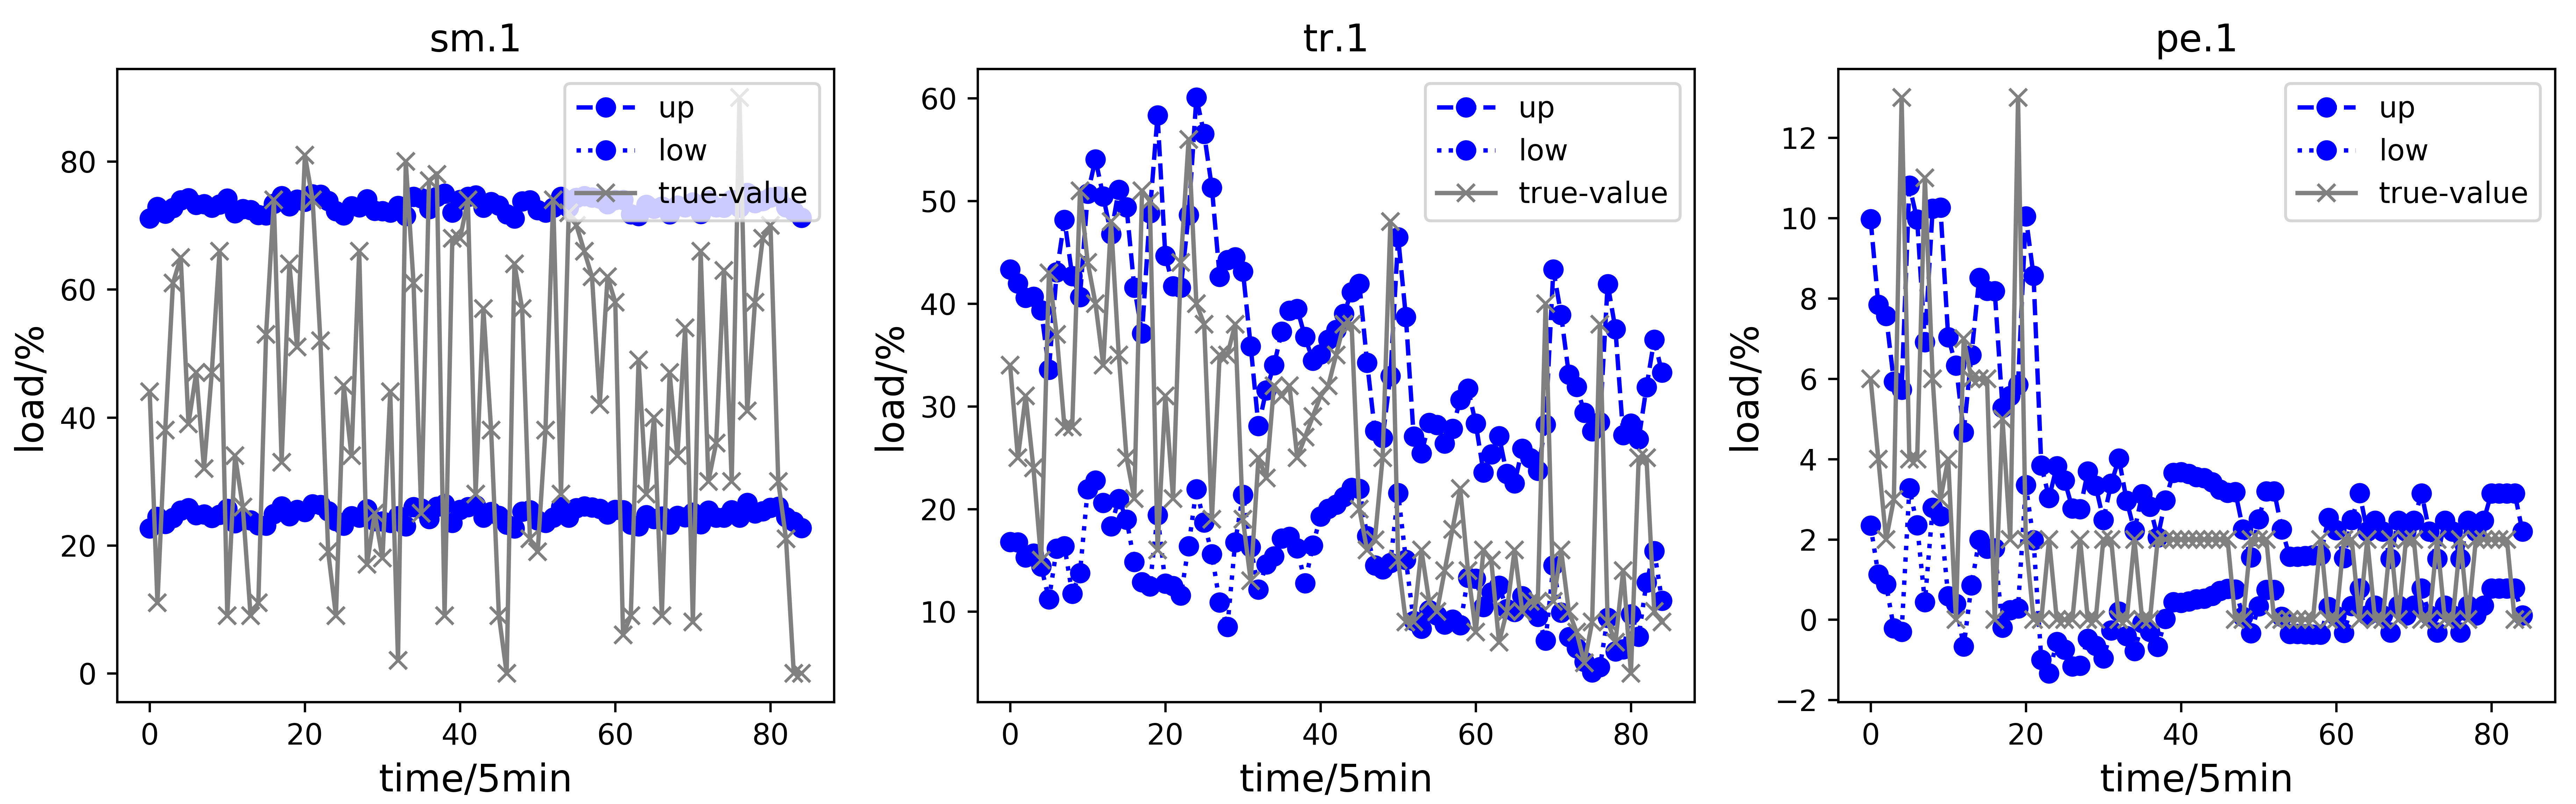
\includegraphics[width=0.65\textwidth]{figures/fig12_a_bayesian.png}
    \caption{Native Bayes预测结果}
    \label{fig:fig12_a}
    \end{figure}
\end{minipage}
\end{frame}

\begin{frame}
\frametitle{实验结果与分析}
\framesubtitle{预测效果分析}
\begin{itemize}
    \item Linear Regression和SVM
\end{itemize}
\begin{minipage}{\textwidth}
    \centering
    \begin{figure}[htb]
    \centering
    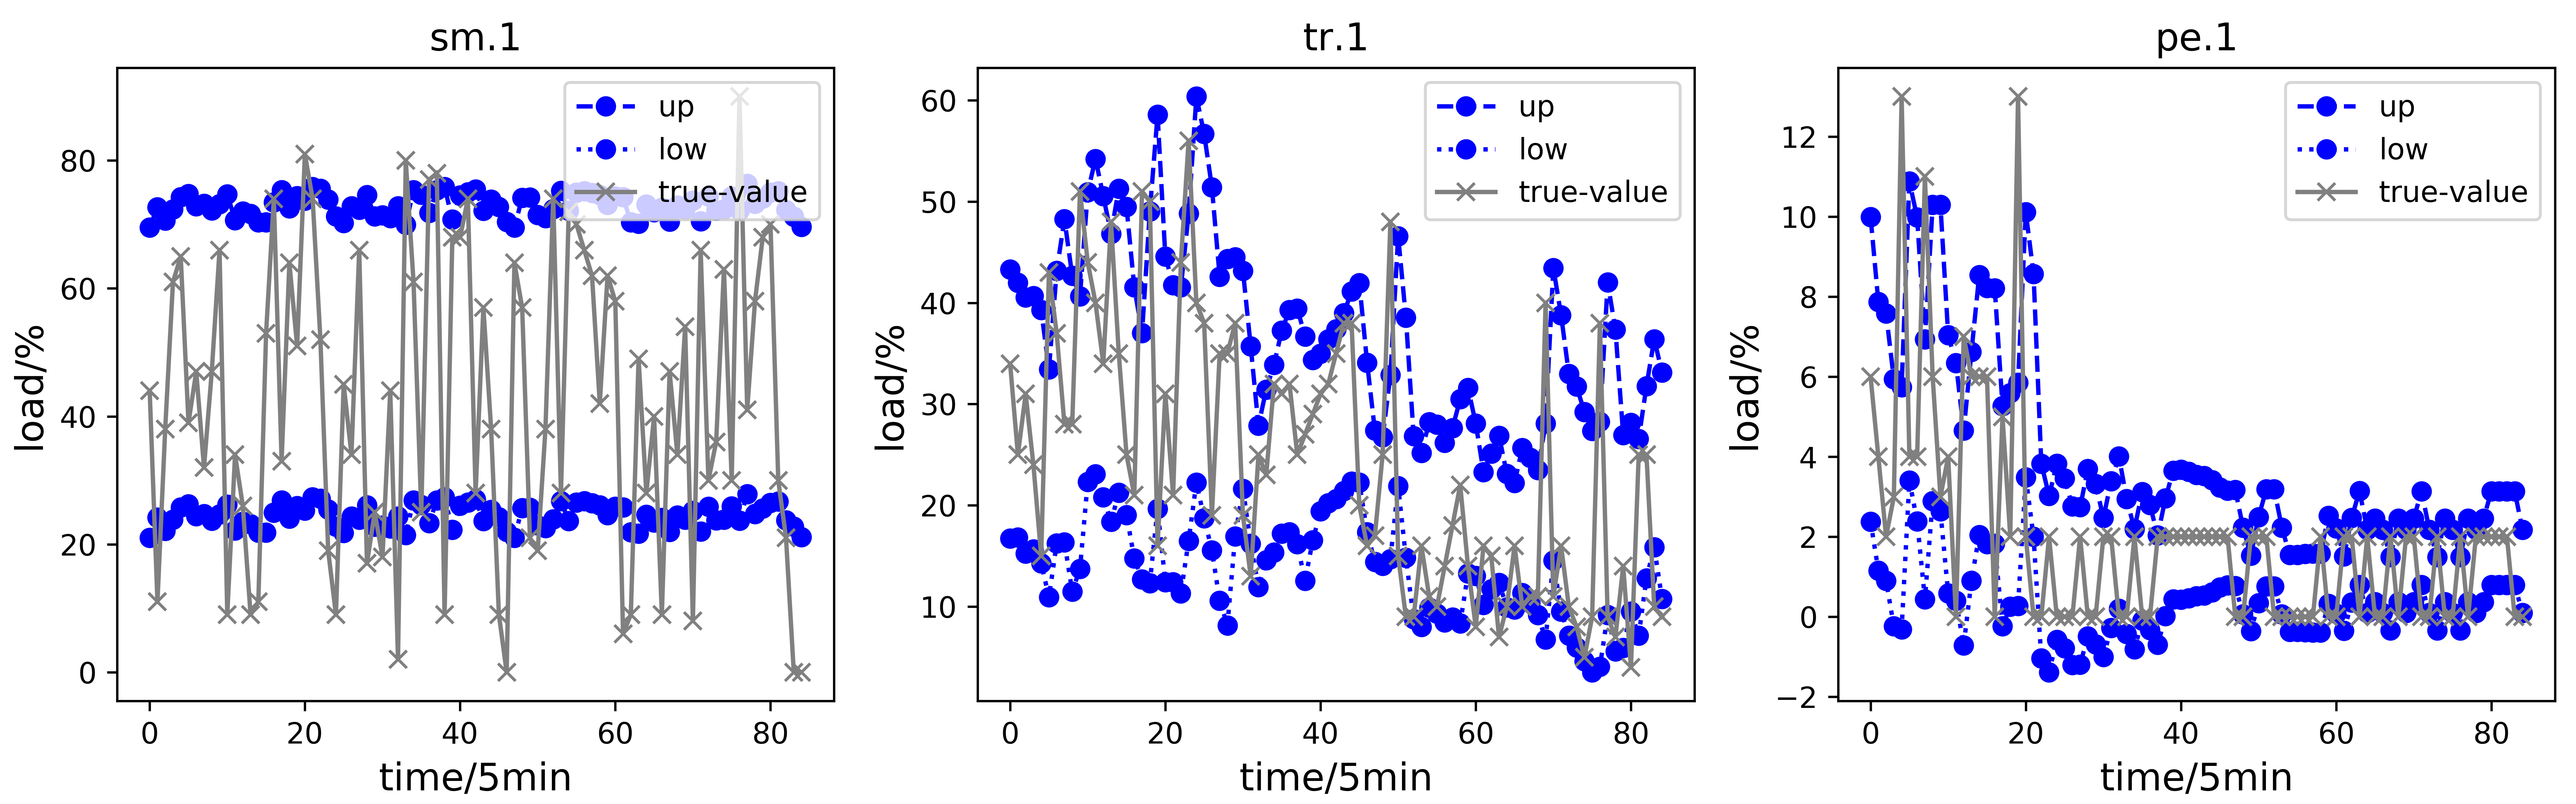
\includegraphics[width=0.65\textwidth]{figures/fig12_b_linear.png}
    \caption{Linear Regression预测结果}
    \label{fig:fig12_b}
    \end{figure}
\end{minipage}
\begin{minipage}{\textwidth}
    \centering
    \begin{figure}[htb]
    \centering
    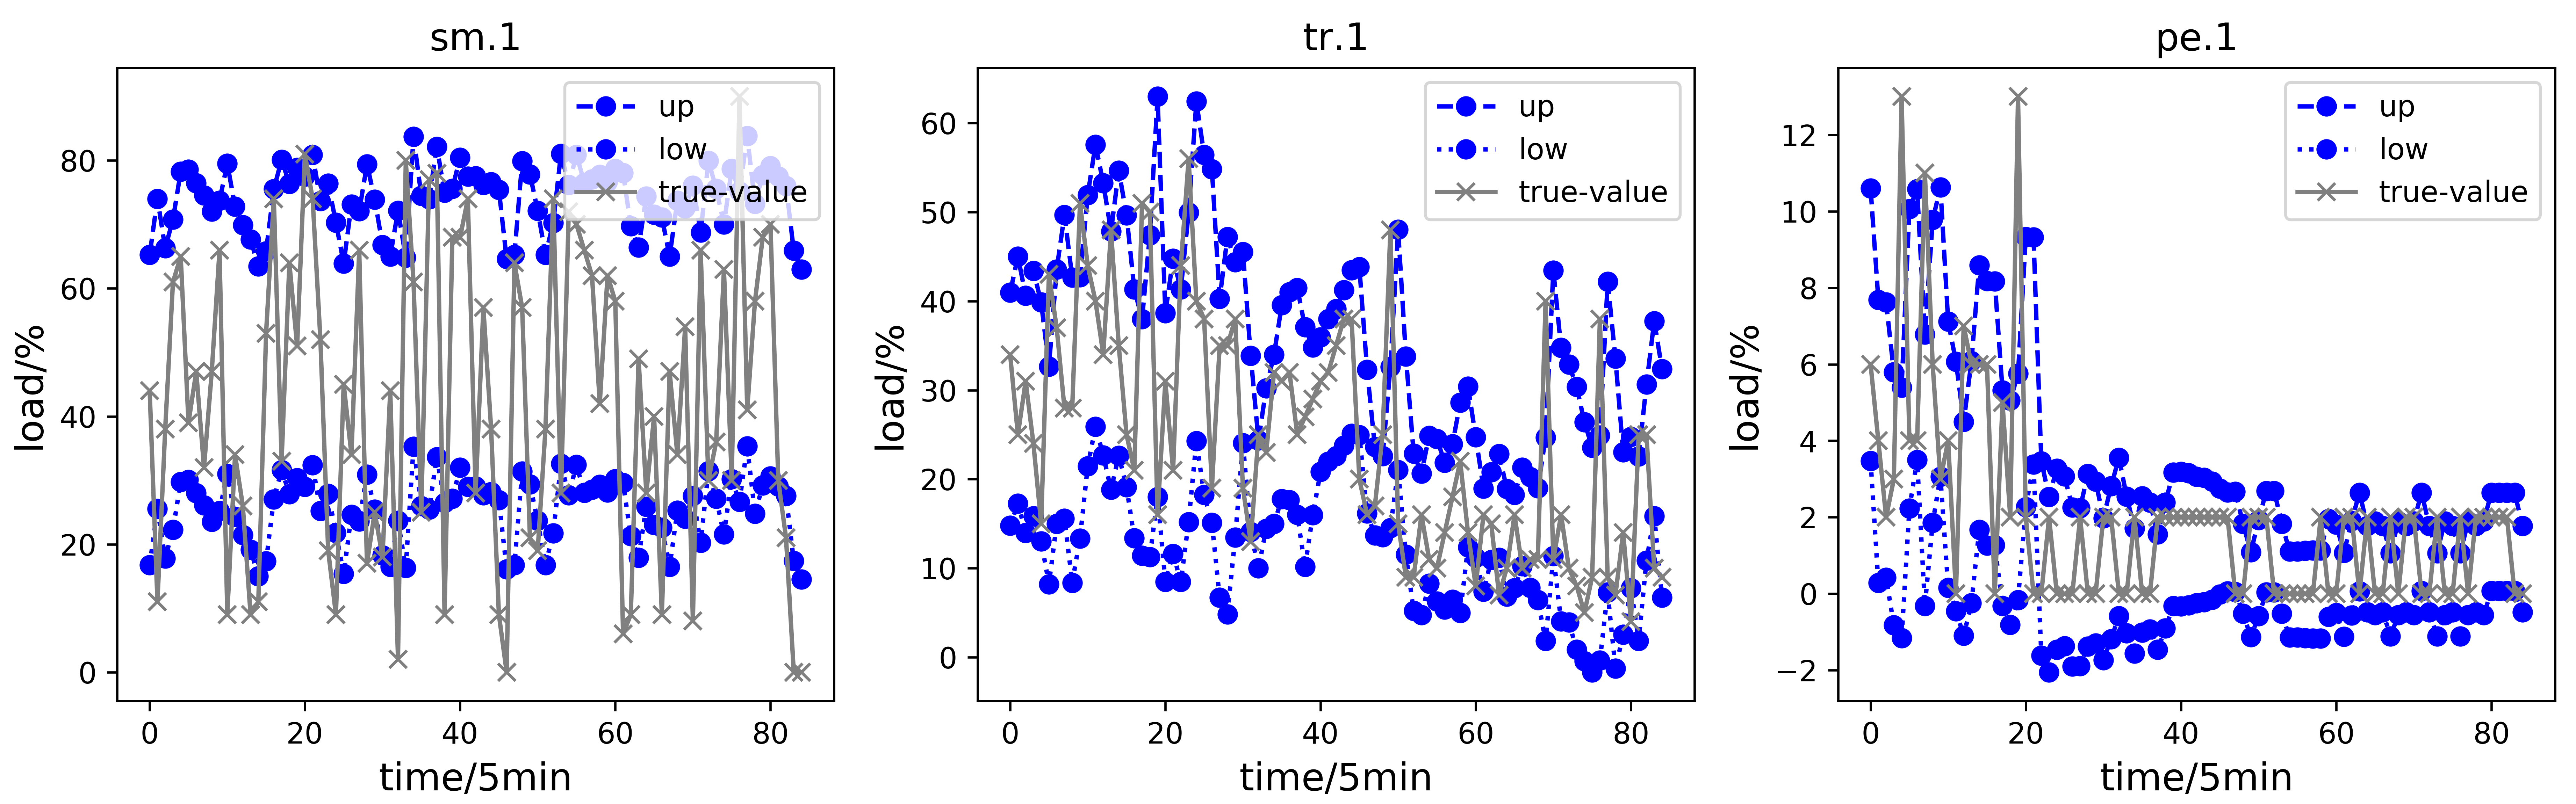
\includegraphics[width=0.65\textwidth]{figures/fig12_c_svm.png}
    \caption{SVM预测结果}
    \label{fig:fig12_c}
    \end{figure}
\end{minipage}
\end{frame}


\begin{frame}
\frametitle{实验结果与分析}
\framesubtitle{预测效果分析}
\begin{itemize}
    \item CART和RFR
\end{itemize}
\begin{minipage}{\textwidth}
    \centering
    \begin{figure}[htb]
    \centering
    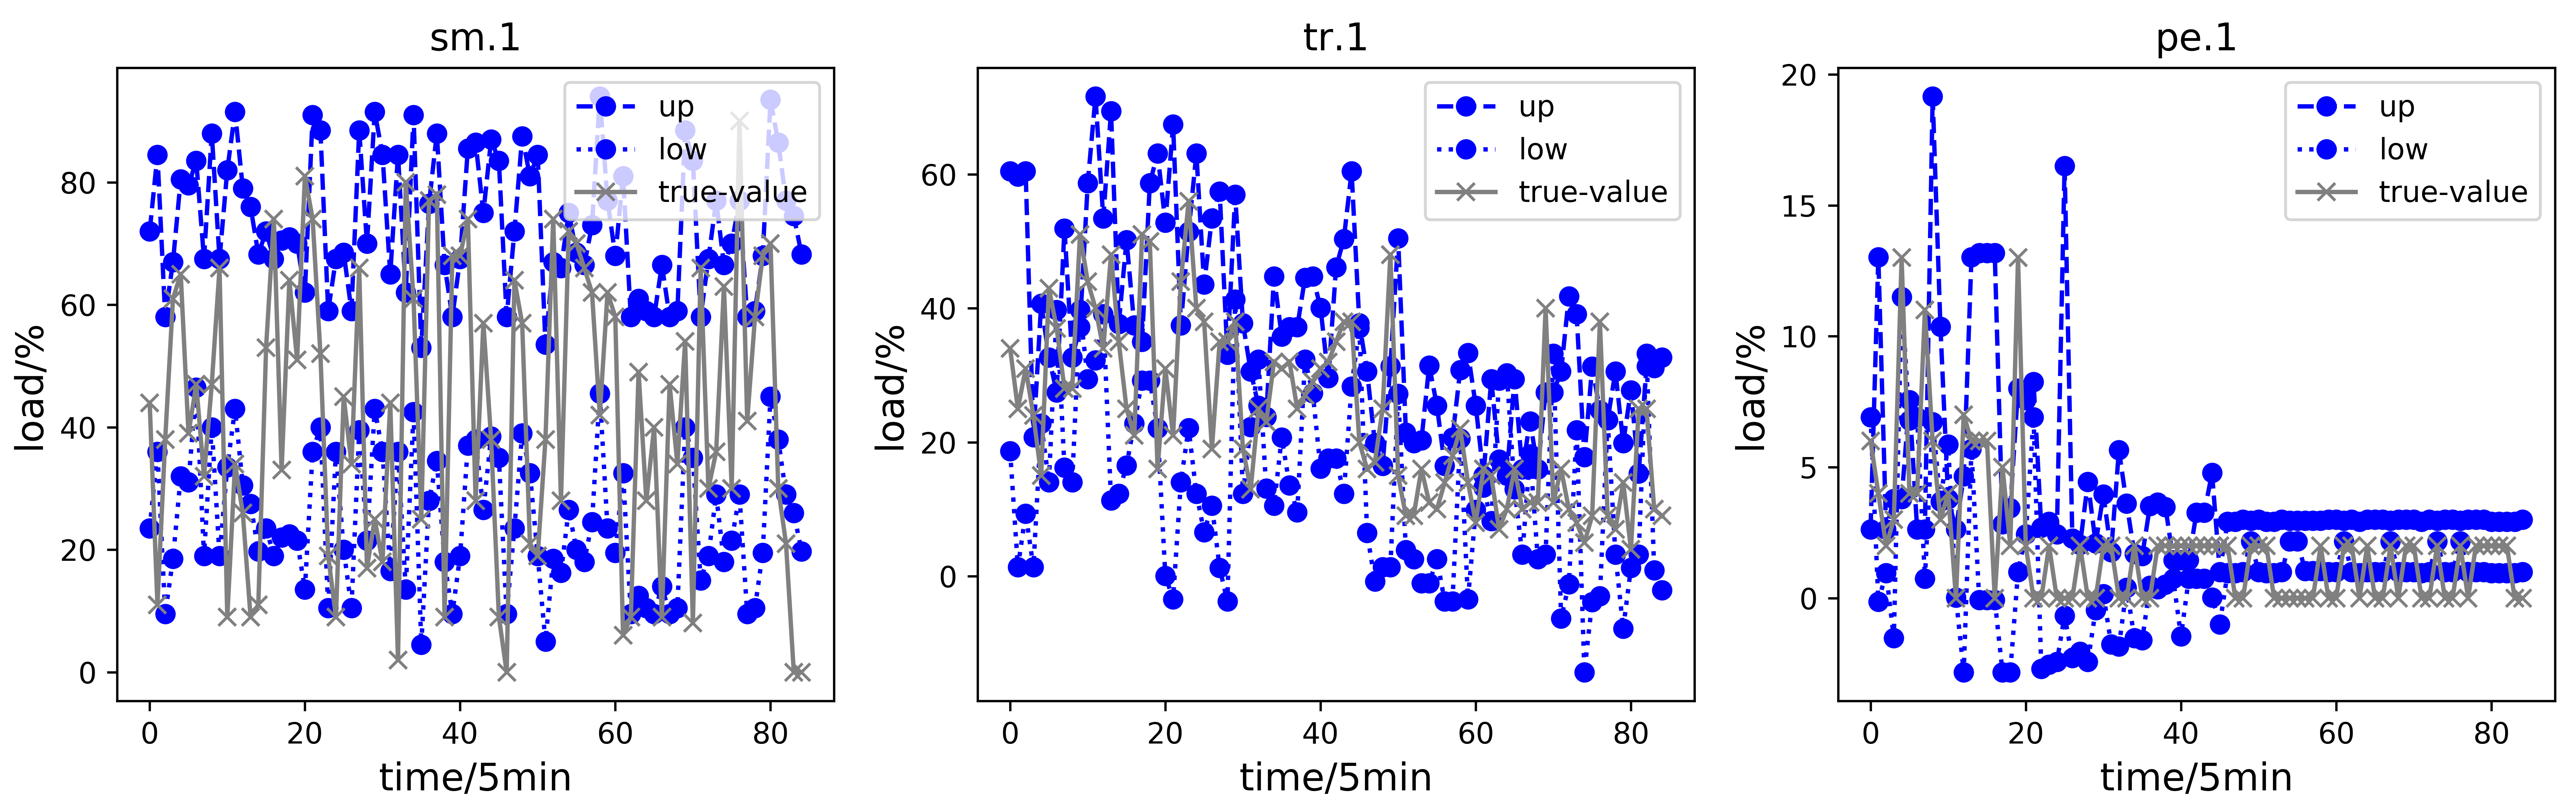
\includegraphics[width=0.65\textwidth]{figures/fig12_d_cart.png}
    \caption{CART预测结果}
    \label{fig:fig12_d}
    \end{figure}
\end{minipage}
\begin{minipage}{\textwidth}
    \centering
    \begin{figure}[htb]
    \centering
    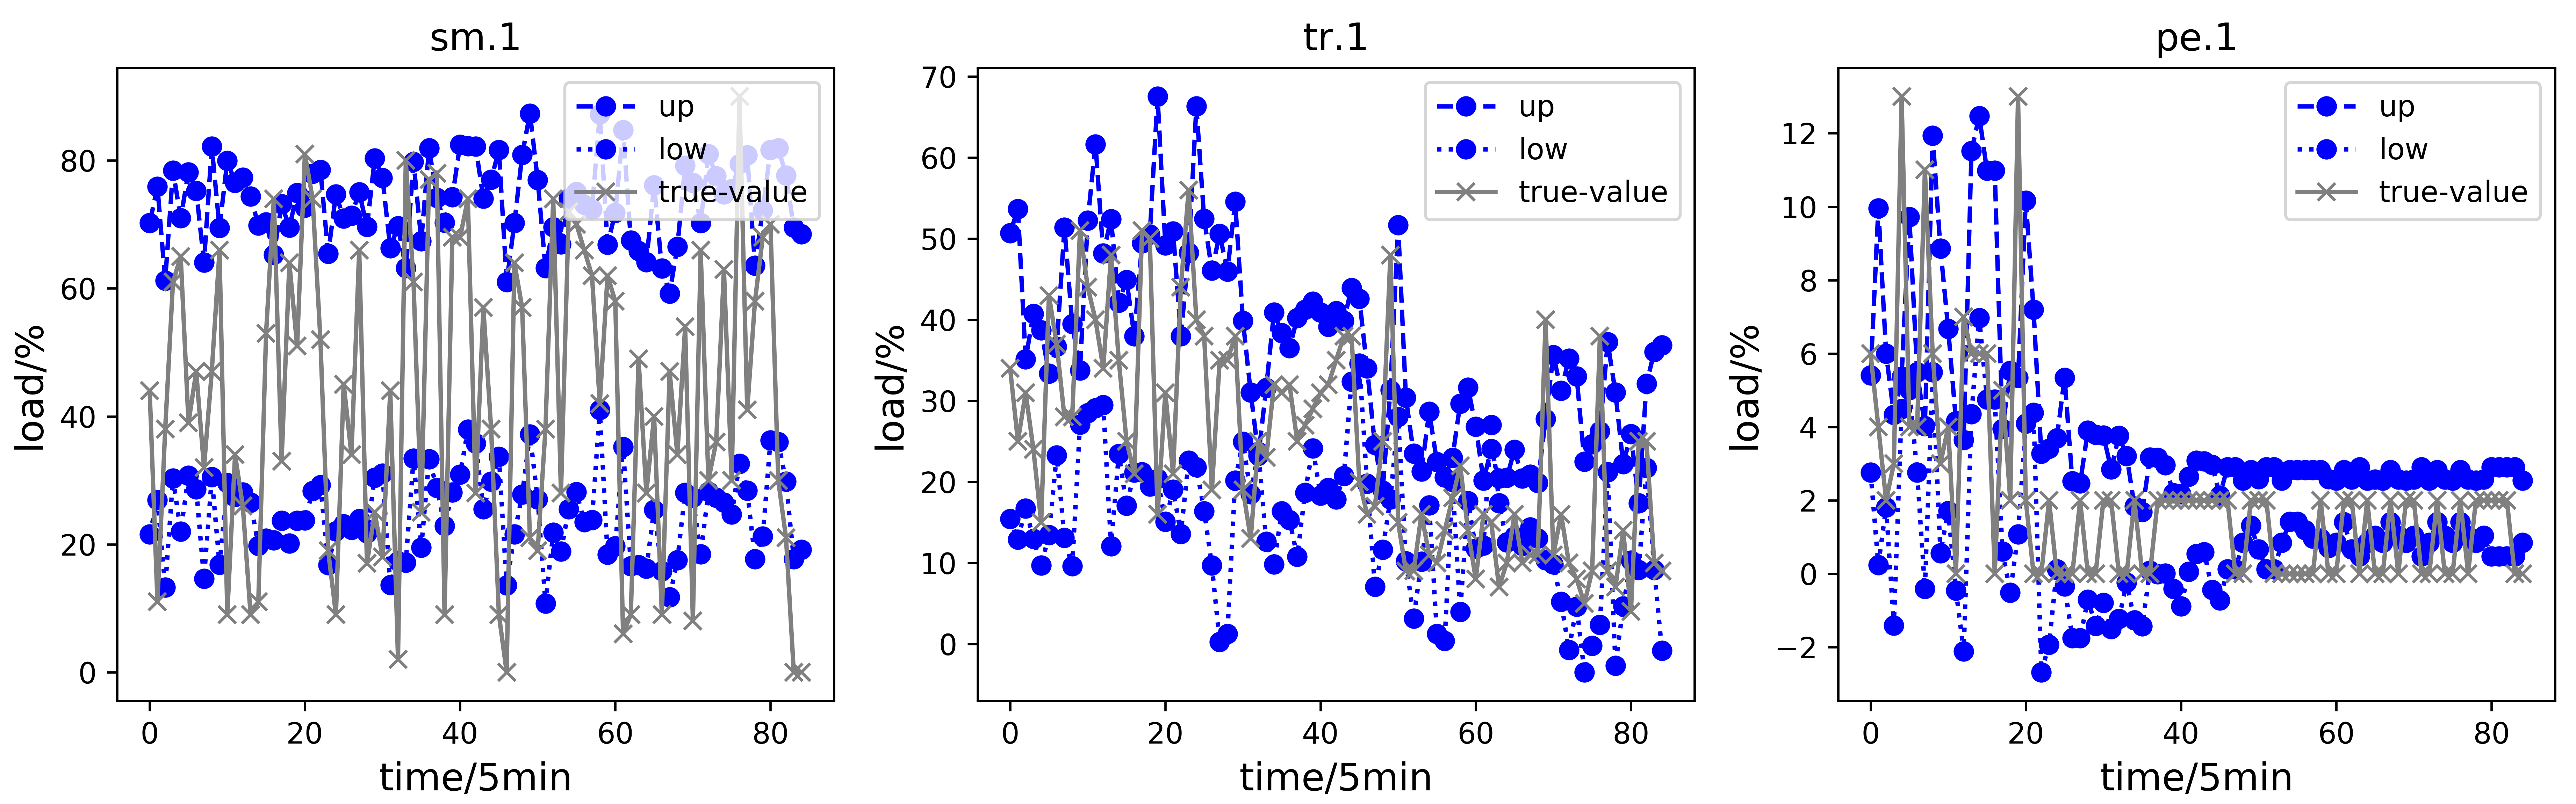
\includegraphics[width=0.65\textwidth]{figures/fig12_e_rfr.png}
    \caption{RFR预测结果}
    \label{fig:fig12_e}
    \end{figure}
\end{minipage}
\end{frame}

\begin{frame}
\frametitle{实验结果与分析}
\framesubtitle{预测准确性对比}
\begin{itemize}
    \item {\color{red}红色:最优}
    \item {\color{yellow}黄色:优}
    \item {\color{blue}蓝色:次优}
\end{itemize}
\begin{table}[hftb]
    \centering
    \resizebox{\textwidth}{!}{%
        \begin{tabular}{cccc}
            \toprule
            \textbf{模型} & \textbf{CWC(\%) $\Downarrow$} & \textbf{PICP(\%) $\Uparrow$} & \textbf{PINEW(\%) $\Downarrow$}\\
            \midrule
            Native Bayes & {\color{blue}71.95} & {\color{yellow}89.41} & {\color{blue}37.41} \\
            Linear Regression & 114 & 83.53 & 40.88 \\
            SVM & 96.92 & 88.24 & 44.19 \\
            CART & 94.16 & 84.31 & {\color{red}34.39} \\
            RFR & {\color{yellow}68.56} & {\color{red}89.42} & 43.55 \\
            SAC-GPSO-SVM & {\color{red}61.26} & {\color{blue}89.40} & {\color{yellow}35.15} \\
            \bottomrule
        \end{tabular}
    }
    \caption{预测准确性对比}
    \label{tab:tab3}
\end{table}
\end{frame}

\begin{frame}
\frametitle{实验结果与分析}
\framesubtitle{预测效率分析}
\begin{itemize}
    \item 剔除超参数优化时间,只考虑模型平均预测时间
\end{itemize}
\begin{figure}[htb]
    \centering
    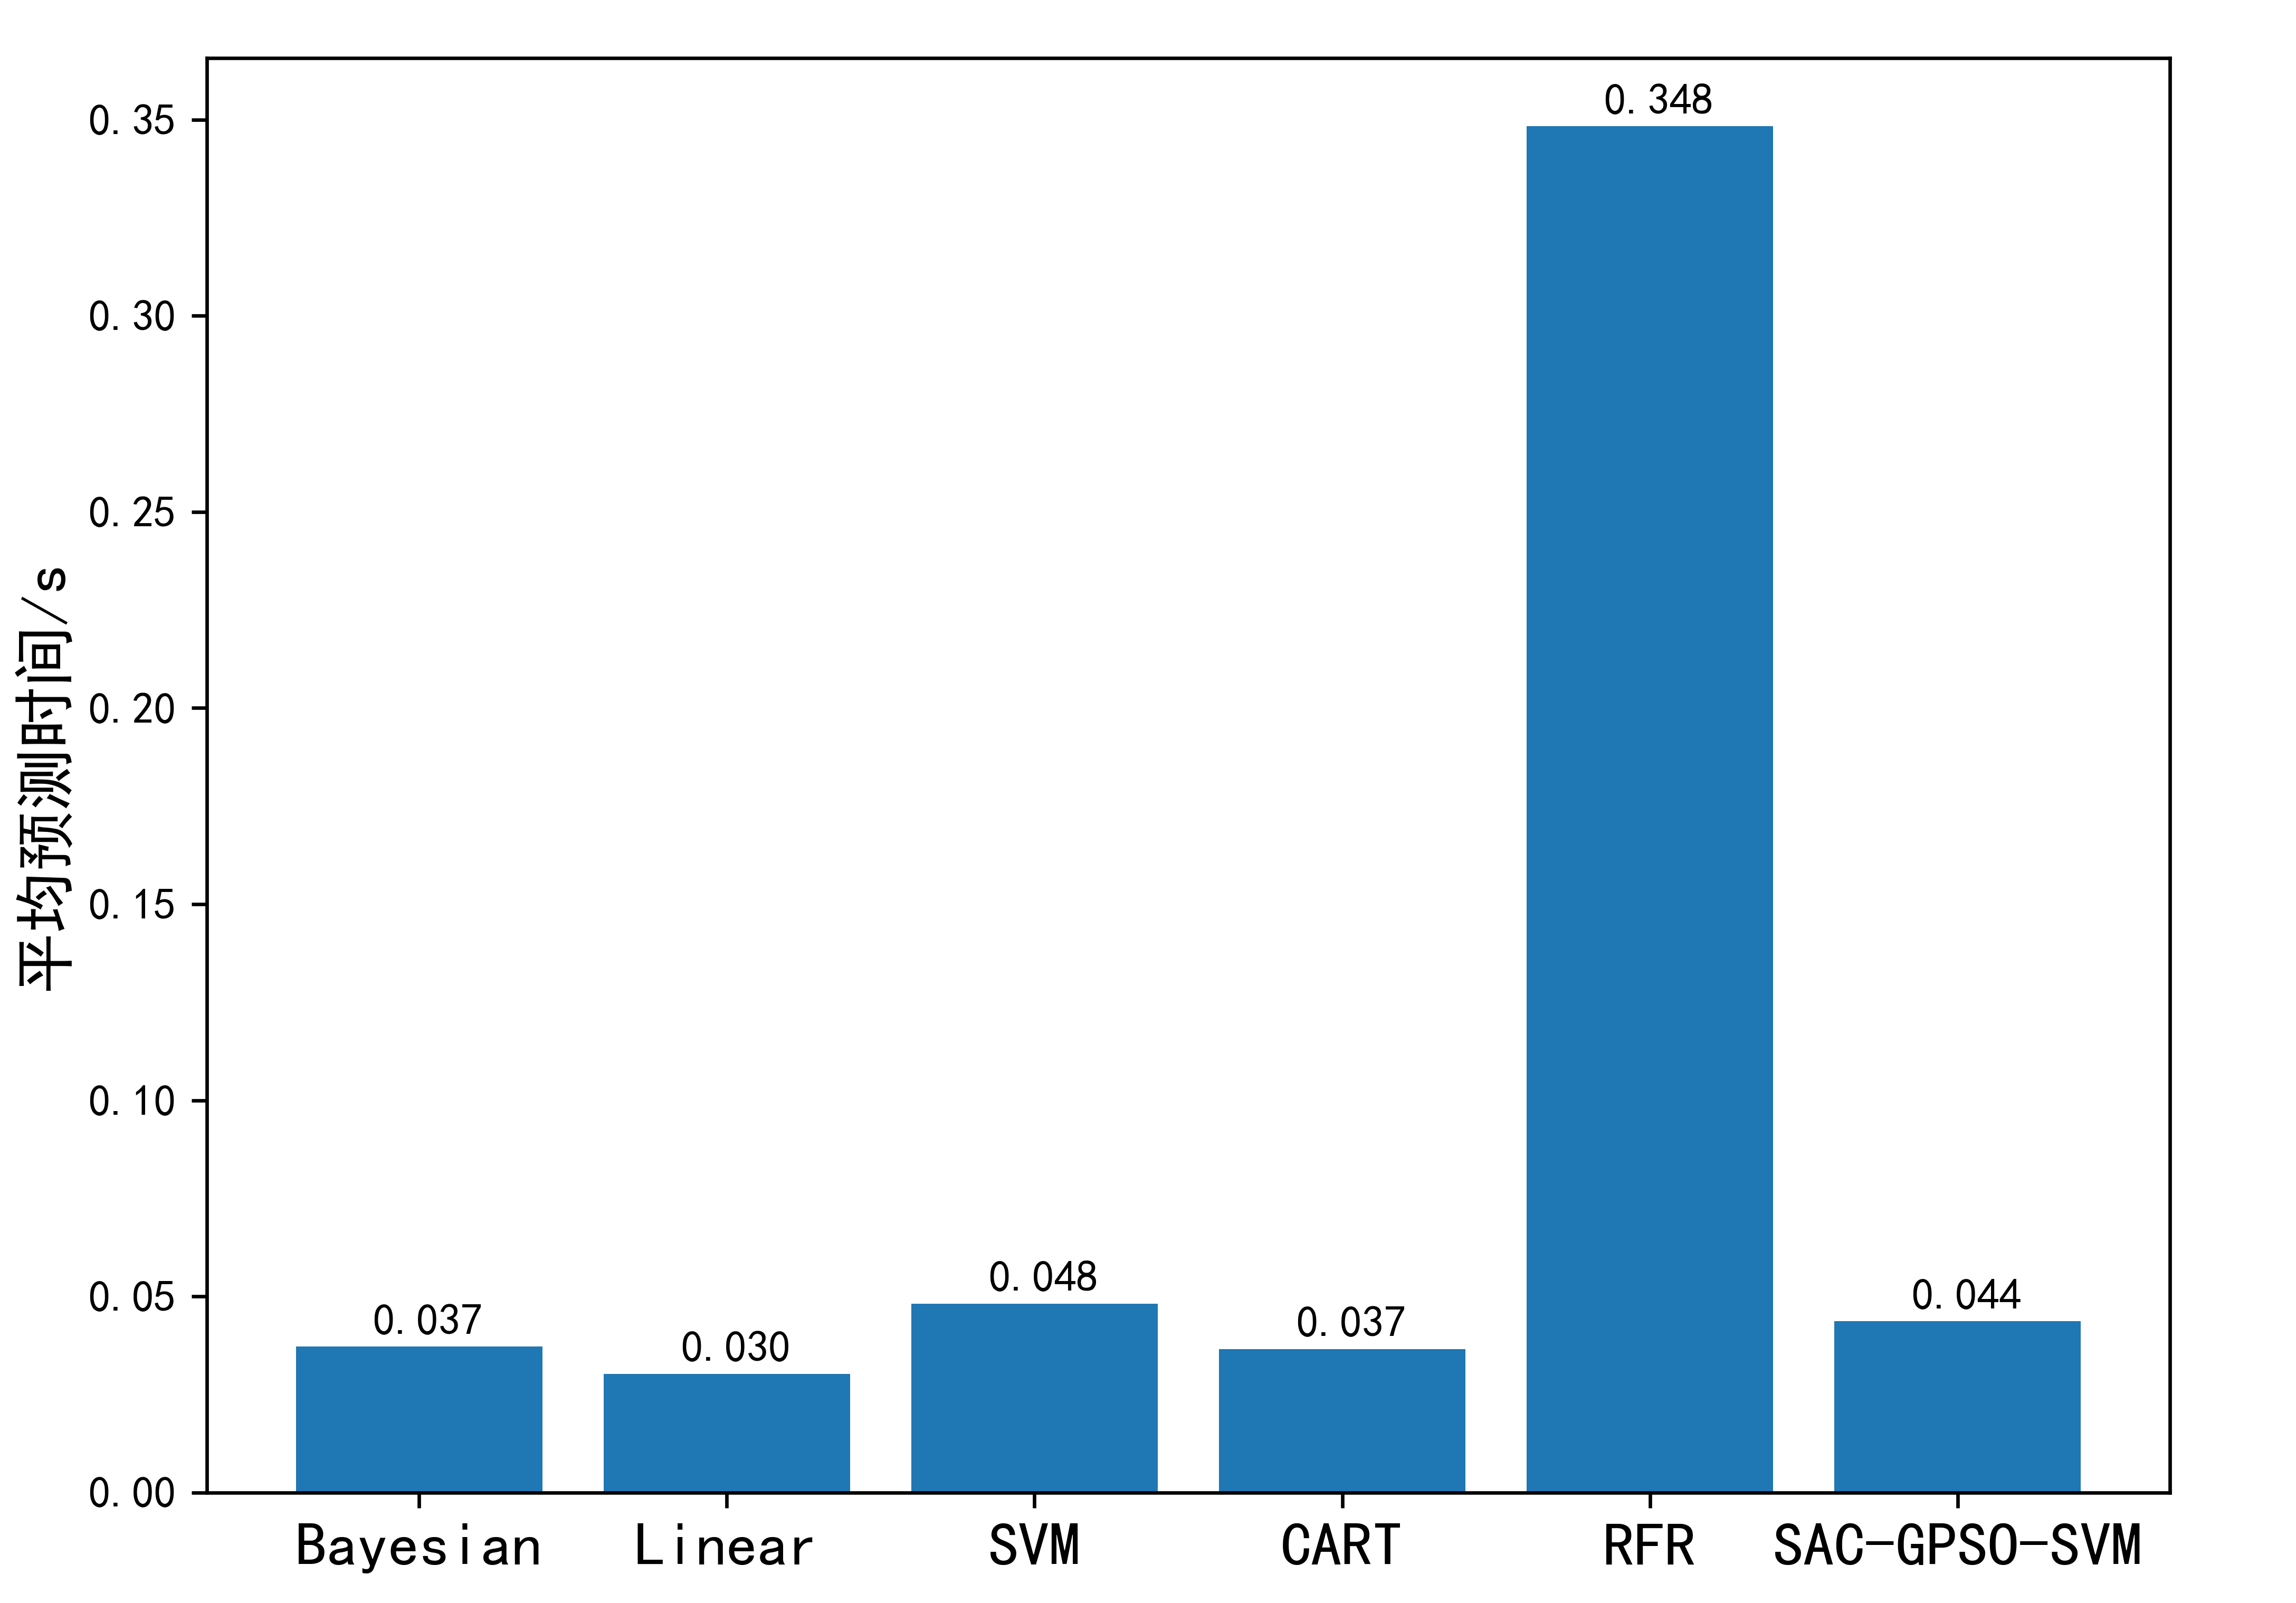
\includegraphics[width=0.75\textwidth]{figures/fig13_time_zh.png}
    \caption{各模型平均预测时间对比}
    \label{fig:fig13}
\end{figure}
\bigskip
\end{frame}

\begin{frame}
\frametitle{实验结果与分析}
\framesubtitle{参数优化效率与模型实时性检验}
\begin{itemize}
    \item {\color{red}红色:最优}
    \item {\color{yellow}黄色:优}
    \item {\color{blue}蓝色:次优}
\end{itemize}
\begin{table}[hftb]
    \centering
    \resizebox{\textwidth}{!}{%
        \begin{tabular}{cccc}
            \toprule
            \textbf{优化方法} & \textbf{平均最优CWC(\%)} & \textbf{平均迭代次数} & \textbf{平均预测时间(s)}\\
            \midrule
            GridSearchCV & {\color{red}68.24} & 1358 & 465.21 \\
            RandomizedSearchCV & {\color{blue}68.56} & {\color{blue}103} & {\color{blue}122.47} \\
            PSO & 68.64 & {\color{yellow}87} & {\color{yellow}78.53} \\
            GPSO & {\color{yellow}68.45} & {\color{red}30} & {\color{red}23.34} \\
            \bottomrule
        \end{tabular}
    }
    \caption{预测准确性对比}
    \label{tab:tab4}
\end{table}
\end{frame}